% ---------------------------------------------------------------------------
%  NewInML @ NeurIPS 2026 -- camera-ready (non-archival).
%
%  Uses the official neurips_2026.sty (2026-01-29) in [final] mode, with the
%  first-page notice replaced by the wording the workshop organisers asked for.
%
%  Every number comes from \input{tables/*}, generated by
%  experiment/make_paper_tables.py from the saved result JSONs. Numbers quoted in
%  the prose come from tables/macros.tex, generated by the same code, so the
%  abstract and the tables cannot disagree. Regenerate before every build.
% ---------------------------------------------------------------------------
\documentclass{article}

\usepackage[final]{neurips_2026}
\makeatletter
\renewcommand{\@noticestring}{NewInML Workshop at the 40th Conference on Neural
  Information Processing Systems (NeurIPS 2026), Paris, France, 2026.}
\makeatother

\usepackage[utf8]{inputenc}
\usepackage[T1]{fontenc}
\usepackage{hyperref}
\hypersetup{pdftitle={What Survives Verification: Steering an Occupation-Gender Stereotype Feature in Two Small Language Models},pdfauthor={Shivam Verma}}
\usepackage{url}
\usepackage{booktabs}
\usepackage{amsmath}
\usepackage{amssymb}
\usepackage{graphicx}
\usepackage{xcolor}
\usepackage{microtype}

% Let TeX stretch interword space a little on stubborn lines rather than run into
% the margin. Standard remedy for sub-10pt overfull hboxes in prose.
\setlength{\emergencystretch}{2em}

\newcommand{\phe}{P(\text{`` he''})}
\newcommand{\pshe}{P(\text{`` she''})}
\newcommand{\pthey}{P(\text{`` they''})}
\newcommand{\ff}[1]{\texttt{f#1}}

\title{What Survives Verification: Steering an\\ Occupation--Gender Stereotype
Feature in Two Small Language Models}

\author{%
  Shivam Verma\\
  Independent researcher\\
  \texttt{shivam.vermaa30@gmail.com}
}

% generated by experiment/make_paper_tables.py -- do not edit
\newcommand{\BDiMSixteenMale}{$-0.27$}
\newcommand{\BDiMTenMale}{$+0.76$}
\newcommand{\BDiMTwelveMale}{$+0.39$}
\newcommand{\BDiMTwentyMale}{$-0.88$}
\newcommand{\BUnembSixteenMale}{$-1.22$}
\newcommand{\BUnembTenMale}{$-0.41$}
\newcommand{\BUnembTwelveMale}{$-0.77$}
\newcommand{\BUnembTwentyMale}{$-1.27$}
\newcommand{\BaseFemale}{$-1.02$}
\newcommand{\BaseFemaleCI}{$[-1.46,-0.59]$}
\newcommand{\BaseMale}{$+2.76$}
\newcommand{\BaseMaleCI}{$[+2.36,+3.14]$}
\newcommand{\BosInflation}{369}
\newcommand{\DlossDiM}{$+1.8\%$}
\newcommand{\DlossDiMSixteen}{$+6.9\%$}
\newcommand{\DlossDiMTen}{$+2.7\%$}
\newcommand{\DlossDiMTwelve}{$+3.8\%$}
\newcommand{\DlossDiMTwenty}{$+11.4\%$}
\newcommand{\DlossProj}{$+2.6\%$}
\newcommand{\DlossSAE}{$+2.3\%$}
\newcommand{\DlossSAEEight}{$+4.1\%$}
\newcommand{\DlossUnembSixteen}{$+4.9\%$}
\newcommand{\DlossUnembTen}{$+2.2\%$}
\newcommand{\DlossUnembTwelve}{$+3.0\%$}
\newcommand{\DlossUnembTwenty}{$+6.4\%$}
\newcommand{\DlossUnembed}{$+1.4\%$}
\newcommand{\GapBase}{$+3.78$}
\newcommand{\GapBaseCI}{$[+3.19,+4.37]$}
\newcommand{\GapDiMEight}{$+3.47$}
\newcommand{\GapDiMEightCI}{$[+2.85,+4.11]$}
\newcommand{\GapDiMSixteen}{$+2.84$}
\newcommand{\GapDiMSixteenCI}{$[+2.22,+3.50]$}
\newcommand{\GapDiMTen}{$+3.34$}
\newcommand{\GapDiMTenCI}{$[+2.72,+3.99]$}
\newcommand{\GapDiMTwelve}{$+3.20$}
\newcommand{\GapDiMTwelveCI}{$[+2.58,+3.86]$}
\newcommand{\GapDiMTwenty}{$+2.37$}
\newcommand{\GapDiMTwentyCI}{$[+1.75,+3.03]$}
\newcommand{\GapSaeEight}{$+0.20$}
\newcommand{\GapSaeEightCI}{$[-0.28,+0.69]$}
\newcommand{\GapSaeFour}{$+2.57$}
\newcommand{\GapSaeFourCI}{$[+2.03,+3.14]$}
\newcommand{\GapSaeSix}{$+1.47$}
\newcommand{\GapSaeSixCI}{$[+1.02,+1.90]$}
\newcommand{\GapUnembEight}{$+2.53$}
\newcommand{\GapUnembEightCI}{$[+2.04,+3.03]$}
\newcommand{\GapUnembSix}{$+2.84$}
\newcommand{\GapUnembSixCI}{$[+2.33,+3.36]$}
\newcommand{\GapUnembSixteen}{$+1.29$}
\newcommand{\GapUnembSixteenCI}{$[+0.95,+1.67]$}
\newcommand{\GapUnembTen}{$+2.20$}
\newcommand{\GapUnembTenCI}{$[+1.75,+2.67]$}
\newcommand{\GapUnembTwelve}{$+1.86$}
\newcommand{\GapUnembTwelveCI}{$[+1.45,+2.31]$}
\newcommand{\GapUnembTwenty}{$+1.00$}
\newcommand{\GapUnembTwentyCI}{$[+0.72,+1.31]$}
\newcommand{\GenChatBase}{74\%}
\newcommand{\GenChatBaseCI}{[60,87]\%}
\newcommand{\GenChatFemBase}{4\%}
\newcommand{\GenChatFemUnembEight}{0\%}
\newcommand{\GenChatFemUnembSix}{1\%}
\newcommand{\GenChatGapBase}{70}
\newcommand{\GenChatGapBaseCI}{[55,84]}
\newcommand{\GenChatGapUnembEight}{21}
\newcommand{\GenChatGapUnembEightCI}{[11,32]}
\newcommand{\GenChatGapUnembSix}{39}
\newcommand{\GenChatGapUnembSixCI}{[26,52]}
\newcommand{\GenChatUnembEight}{21\%}
\newcommand{\GenChatUnembEightCI}{[11,32]\%}
\newcommand{\GenChatUnembSix}{40\%}
\newcommand{\GenChatUnembSixCI}{[26,53]\%}
\newcommand{\GenNOcc}{31}
\newcommand{\GenNPerCond}{630}
\newcommand{\GenRawBase}{89\%}
\newcommand{\GenRawBaseCI}{[83,95]\%}
\newcommand{\GenRawFemBase}{22\%}
\newcommand{\GenRawFemUnembEight}{3\%}
\newcommand{\GenRawFemUnembSix}{4\%}
\newcommand{\GenRawGapBase}{67}
\newcommand{\GenRawGapBaseCI}{[52,79]}
\newcommand{\GenRawGapUnembEight}{19}
\newcommand{\GenRawGapUnembEightCI}{[10,29]}
\newcommand{\GenRawGapUnembSix}{33}
\newcommand{\GenRawGapUnembSixCI}{[22,45]}
\newcommand{\GenRawUnembEight}{22\%}
\newcommand{\GenRawUnembEightCI}{[13,32]\%}
\newcommand{\GenRawUnembSix}{37\%}
\newcommand{\GenRawUnembSixCI}{[26,48]\%}
\newcommand{\HeldBase}{$+2.52$}
\newcommand{\HeldBaseCI}{$[+2.31,+2.74]$}
\newcommand{\HeldGapBase}{$+4.34$}
\newcommand{\HeldGapBaseCI}{$[+3.91,+4.77]$}
\newcommand{\HeldGapDiMSix}{$+4.09$}
\newcommand{\HeldGapDiMSixCI}{$[+3.59,+4.60]$}
\newcommand{\HeldGapSaeSix}{$+2.09$}
\newcommand{\HeldGapSaeSixCI}{$[+1.62,+2.59]$}
\newcommand{\HeldGapUnembSix}{$+3.34$}
\newcommand{\HeldGapUnembSixCI}{$[+2.97,+3.72]$}
\newcommand{\HeldSteer}{$-0.53$}
\newcommand{\HeldSteerCI}{$[-0.73,-0.34]$}
\newcommand{\LfmBaseFemale}{$-2.43$}
\newcommand{\LfmBaseFemaleCI}{$[-2.99,-1.86]$}
\newcommand{\LfmBaseMale}{$+1.22$}
\newcommand{\LfmBaseMaleCI}{$[+0.73,+1.73]$}
\newcommand{\LfmRankOneSwing}{+0.29}
\newcommand{\LfmRankTwoSwing}{3.16}
\newcommand{\PrimaryMaxHolm}{2.9\times10^{-3}}
\newcommand{\PrimaryN}{11}
\newcommand{\ProjGapHeldBase}{$+4.34$}
\newcommand{\ProjGapHeldBaseCI}{$[+3.91,+4.77]$}
\newcommand{\ProjGapHeldDiM}{$+3.21$}
\newcommand{\ProjGapHeldDiMCI}{$[+2.73,+3.72]$}
\newcommand{\ProjGapHeldSae}{$+2.62$}
\newcommand{\ProjGapHeldSaeCI}{$[+2.17,+3.07]$}
\newcommand{\ProjGapTplBase}{$+3.78$}
\newcommand{\ProjGapTplBaseCI}{$[+3.19,+4.37]$}
\newcommand{\ProjGapTplDiM}{$+2.28$}
\newcommand{\ProjGapTplDiMCI}{$[+1.78,+2.77]$}
\newcommand{\ProjGapTplSae}{$+2.03$}
\newcommand{\ProjGapTplSaeCI}{$[+1.52,+2.57]$}
\newcommand{\ProjHeld}{$-0.20$}
\newcommand{\ProjHeldCI}{$[-0.38,-0.02]$}
\newcommand{\ProjTpl}{$+0.27$}
\newcommand{\ProjTplCI}{$[+0.11,+0.43]$}
\newcommand{\ReproMaxErr}{1.4\times10^{-5}}
\newcommand{\RobBase}{$+2.75$}
\newcommand{\RobBaseCI}{$[+1.92,+3.51]$}
\newcommand{\RobDelta}{$-3.29$}
\newcommand{\RobSteer}{$-0.54$}
\newcommand{\RobSteerCI}{$[-1.10,-0.11]$}
\newcommand{\SteerMale}{$+0.09$}
\newcommand{\SteerMaleCI}{$[-0.07,+0.25]$}
\newcommand{\ValidChatN}{40}
\newcommand{\ValidChatRho}{0.81}
\newcommand{\ValidRawN}{40}
\newcommand{\ValidRawRho}{0.80}
\newcommand{\XBaseFemale}{$+0.02$}
\newcommand{\XBaseFemaleCI}{$[-0.58,+0.60]$}
\newcommand{\XBaseMale}{$+2.37$}
\newcommand{\XBaseMaleCI}{$[+1.99,+2.73]$}
\newcommand{\XDiMMinusEightFemale}{$-1.82$}
\newcommand{\XDiMMinusEightFemaleCI}{$[-2.41,-1.25]$}
\newcommand{\XDiMMinusEightMale}{$+0.33$}
\newcommand{\XDiMMinusEightMaleCI}{$[+0.02,+0.63]$}
\newcommand{\XFrames}{6}
\newcommand{\XGapBase}{$+2.35$}
\newcommand{\XGapBaseCI}{$[+1.65,+3.07]$}
\newcommand{\XGapDiMEight}{$+2.15$}
\newcommand{\XGapDiMEightCI}{$[+1.50,+2.82]$}
\newcommand{\XGapUnembEight}{$+1.56$}
\newcommand{\XGapUnembEightCI}{$[+1.05,+2.08]$}
\newcommand{\XGapUnembSix}{$+1.75$}
\newcommand{\XGapUnembSixCI}{$[+1.19,+2.32]$}
\newcommand{\XNFemale}{20}
\newcommand{\XNMale}{20}
\newcommand{\XOverlap}{9}
\newcommand{\XProjDiMFemale}{$-0.24$}
\newcommand{\XProjDiMFemaleCI}{$[-0.74,+0.25]$}
\newcommand{\XProjDiMMale}{$+1.45$}
\newcommand{\XProjDiMMaleCI}{$[+1.16,+1.73]$}
\newcommand{\XUnembMinusEightFemale}{$-2.24$}
\newcommand{\XUnembMinusEightFemaleCI}{$[-2.69,-1.80]$}
\newcommand{\XUnembMinusEightMale}{$-0.68$}
\newcommand{\XUnembMinusEightMaleCI}{$[-0.93,-0.43]$}
\newcommand{\XUnembMinusSixFemale}{$-1.87$}
\newcommand{\XUnembMinusSixFemaleCI}{$[-2.36,-1.39]$}
\newcommand{\XUnembMinusSixMale}{$-0.13$}
\newcommand{\XUnembMinusSixMaleCI}{$[-0.39,+0.14]$}


\begin{document}
\maketitle

\begin{abstract}
Bias-mitigation recipes increasingly work by naming an internal object: ablate this
direction, clamp that sparse-autoencoder (SAE) feature. Our contribution is a
\emph{verification protocol} for such recipes, not a better debiasing method, together
with what the protocol changed when we applied it, on a laptop, to an
occupation$\rightarrow$pronoun stereotype in Llama-3.2-1B-Instruct and LFM2.5-230M. The
protocol requires two independent lines of evidence per candidate feature, then tests the
survivor for sufficiency, necessity, transfer and specificity against matched-norm
baselines. In Llama, subtracting one feature (\ff{32258}) moves the
he--she log-odds on male-stereotyped occupations from \BaseMale{} \BaseMaleCI{} to
\SteerMale{} \SteerMaleCI{}, an interval containing parity. The effect holds on 24
occupations under template families never used for discovery, and projecting the
direction out removes most of the bias (\HeldBase{}${}\to{}$\ProjHeld{} on held-out
occupations).

Verification also changed what we claim. Which direction debiases best depends on the
metric. The raw unembedding direction reaches parity on male-stereotyped occupations more
cheaply (\DlossUnembed{} against \DlossSAE{} WikiText loss), but by moving every
occupation toward `` she''. Only the SAE feature closes the gap between male- and
female-stereotyped occupations (\GapBase{}${}\to{}$\GapSaeEight{} \GapSaeEightCI{}).
The feature is a masculine-referent feature rather than a stereotype feature, so its effect
is asymmetric. On 40 further occupations and in sampled text, next-token log-odds order
occupations as generation does (Spearman $\rho={}$\ValidRawRho), but understate the
female-side stereotype. A discovery ranking is not a causal ranking either: in LFM2.5 the
top-ranked masculine candidate is inert while the rank-2 candidate swings the bias by
\LfmRankTwoSwing{} log-odds, which overturned a cross-model claim we had drawn from
rank~1. We also document two silent SAE failure modes, corrupt normalisation statistics
and beginning-of-sequence contamination that inflates reconstruction error
\BosInflation$\times$, and give a pre-flight checklist that catches both.
\end{abstract}

\section{Introduction}

That a language model continues ``The mechanic said that'' with `` he'' and ``The nurse
said that'' with `` she'' is not news; it has been measured since static word embeddings
\citep{bolukbasi2016,caliskan2017} and formalised into coreference benchmarks
\citep{rudinger2018,zhao2018}. Newer is the claim that the behaviour can be
\emph{located}: attributed to identifiable internal components and then edited
\citep{vig2020,marks2024}. That promise is attractive because it offers surgical edits
instead of retraining.

It also carries an assumption that is rarely stated: that the internal object a recipe
names is stable. Stable across models, so a direction found in one transfers; and stable
within a model, so the feature a discovery method ranks first is the one that drives the
behaviour. This paper tests both, end to end on a consumer laptop with public SAEs, and
finds that the second assumption is the one that fails first.

\paragraph{Contributions.}
\textbf{(i)} A two-test discovery criterion, activation selectivity plus decoder-level
output push, which rejects the impostors either test admits alone: a
``food'' feature riding on \emph{dietitian}, and a possessive-determiner feature
(\S\ref{sec:discovery}). \textbf{(ii)} A causal result reported with intervals rather
than ratios, verified on occupations and templates held out from discovery, and tested for
\emph{necessity} as well as sufficiency by projecting the direction out
(\S\ref{sec:dose}--\S\ref{sec:ablation}). \textbf{(iii)} A matched-norm baseline suite on
two bias--capability frontiers. A two-line unembedding baseline beats the feature on one
group's parity, but only the feature removes the occupation dependence
(\S\ref{sec:baselines}). Expanded probes and a generation-level evaluation test the metric
itself (\S\ref{sec:beyond}). \textbf{(iv)} Evidence that a discovery ranking is a weak
predictor of causal effect, including the cross-model claim of our own that it overturns
(\S\ref{sec:crossmodel}). \textbf{(v)} Two silent SAE failure modes, corrupt
normalisation statistics and beginning-of-sequence contamination that inflates
reconstruction error by $369\times$, plus the pre-flight check that catches both
(\S\ref{sec:preflight}).

None of the ingredients here are new: SAEs, activation steering, dose--response sweeps and
difference-in-means all come from prior work (\S\ref{sec:related}). What we contribute is
a verification protocol, run to the same depth in both models, and what that verification
changed. It is not a better debiasing method; \S\ref{sec:baselines} shows that whether the
feature even beats a two-line baseline depends on how the stereotype is scored. Code, probe sets and every per-prompt
measurement are at
\url{https://github.com/Photon3009/stereotype-feature-steering-experiment}.
Two models cannot support a claim about how often anything happens, and we make none. What
two models plus a systematic search do support is narrower. The object such a recipe names
is not stable, so the recipe has to be re-verified wherever it is applied, and a null
result about it needs a search before it can be reported as an absence.

\section{Setup}
\label{sec:setup}

\paragraph{Models and SAEs.}
Llama-3.2-1B-Instruct (16 layers, $d_{\text{model}}=2048$) with a public
$32{,}768$-feature SAE on the layer-8 residual stream, and LFM2.5-230M (a different
architecture, 14 layers) with public SAEs on layers 5 and 9. Layer 8 is the network
midpoint; the trace in Appendix~\ref{app:trace} shows the pronoun prediction is not yet
resolved there, and that ablating layers 9--14, immediately downstream, is what destroys
it. Analysis runs on CPU in \texttt{float32} via TransformerLens
\citep{nanda2022transformerlens}; held-out text is WikiText-103
\citep{merity2016wikitext}. Public SAE coverage, not choice, fixes the layer, a
constraint we return to in \S\ref{sec:limitations}.

\paragraph{Probes.}
All prompts end immediately before a pronoun, so the stereotype is one next-token
distribution. \emph{Discovery:} 36 templates ``The \{occupation\} said that'', 12
male-stereotyped, 12 female-stereotyped and 12 neutral, in which only the occupation word
differs, so contrasts cannot be driven by topic. \emph{Held out:} 24 occupations appearing
nowhere in discovery, under two unseen template families. \emph{Context override:} 24
counter-stereotypical prompts containing an explicit pronoun (``The mechanic tied
\textbf{her} hair back before''). Stereotype assignments follow
\citet{zhao2018,rudinger2018}; lists in Appendix~\ref{app:probes}.

\paragraph{Metric.}
Per prompt we use the pronoun log-odds $b = \log \phe - \log \pshe$: signed, symmetric
about parity, and, unlike a ratio of group-mean probabilities, pairable across steering
strengths, because the same occupation appears at every strength. We report
group means with $95\%$ bootstrap CIs over prompts ($20{,}000$ resamples) and the
group-mean probabilities, so results stay comparable with ratio-style reporting.
Appendix~\ref{app:specificity} reports what else the model puts mass on, so a reader can
judge whether a two-token log-odds tracks its behaviour.

\paragraph{Steering.}
Feature $i$'s decoder direction, mapped out of the SAE's normalised space, is
$d_i = W^{\text{dec}}_i \odot \sigma$ for normalisation standard deviations $\sigma$. We
add $s\,d_i$ to the layer-8 residual stream at every position and read the next-token
distribution, sweeping $s$. One dose unit is $\lVert d_{32258}\rVert$, which is $2.0\%$
of the mean layer-8 residual norm, so even $|s|=8$ perturbs the stream by about $16\%$ of
its norm. Competing directions in \S\ref{sec:baselines} are rescaled to the same norm, so
a given $s$ is an equally sized perturbation for every method.

\paragraph{Statistics.}
Primary inference is on effect sizes with CIs; we also report two-sided Wilcoxon
signed-rank tests paired by occupation. Holm correction is applied to a named
family of \PrimaryN{} tests, the ones the text draws a conclusion from (steering at
$s=-6$ on the discovery, varied-predicate and held-out sets; steering at $s=+6$ on the
female-stereotyped set; projection on both sets; context override; the negative control; and the expanded-probe
and two generation tests of \S\ref{sec:beyond}).
All \PrimaryN{} survive (largest adjusted $p={}\PrimaryMaxHolm$), the negative control
included. Sweep-table $p$-values are uncorrected. Two cautions. With $n=12$ pairs the smallest attainable two-sided $p$ is
$4.9\times10^{-4}$, so a test at that value is at the floor, and the floor is not
evidence of a large effect. And because the models are deterministic and the same
occupations recur at every strength, the test easily calls negligible shifts significant.
Our negative control (\S\ref{sec:controls}) is exactly that, which is why effect size,
not $p$, is the decision variable.

\section{Pre-flight: an SAE can fail silently in both directions}
\label{sec:preflight}

We report this first because it invalidated our own first round of results.

The layer-8 SAE was trained on standardised inputs, with per-dimension means and standard
deviations shipped in a separate file. That file was corrupt. Fed raw residuals, the
encoder's pre-activations almost never clear its threshold: mean $L_0 = 3$ of
$32{,}768$. Fed the corrupt statistics, a different code path produced the opposite
pathology, $L_0 = 30{,}688$: a ``sparse'' autoencoder with $94\%$ of features active.
Neither raised a warning. One silently reports that nothing is happening, the other that
everything is. This is train/serving skew from a mislaid scaler, transplanted into
interpretability, where the symptom is a plausible-looking null result.

\begin{table}[t]
\centering
\caption{SAE pre-flight at layer 8: same SAE, same inputs, only the normalisation
statistics differ. $L_0$ and FVU are measured on 100 held-out WikiText passages,
excluding the first positions of each (see below).}
\label{tab:preflight}
\small
\begin{tabular}{lrrrl}
\toprule
normalisation statistics & mean $L_0$ & \% active & median FVU & reading \\
\midrule
raw inputs, unstandardised    & 3        & 0.01\% & ---   & dead \\
corrupt file from the catalog & 30{,}688 & 93.7\% & ---   & saturated \\
reconstructed from WikiText   & 3{,}596 & 11.0\% & 0.157 & usable, but not sparse \\
\midrule
\emph{as above, BOS included} & 4{,}033 & 12.3\% & 58.1 & unusable diagnostic \\
\bottomrule
\end{tabular}
\end{table}

\paragraph{Two numbers, not one.}
Reconstructing the statistics from WikiText with Welford's algorithm gives
Table~\ref{tab:preflight}: the SAE reconstructs well (median FVU $0.157$, so $\approx
84\%$ of variance explained) while being far from sparse ($11.0\%$ of features active
where hundreds would be expected). Those facts point opposite ways, and only reporting
both makes the operating point legible. $L_0$ alone suggests a broken SAE; FVU alone
suggests a healthy one.

\paragraph{A second silent failure: BOS.}
The last row differs from the third only in whether the beginning-of-sequence position is
included. Its residual norm dwarfs every other position's and dominates any aggregate:
FVU inflates $369\times$, and the maximally activating context of \emph{every} feature we
examined was BOS or the token after it.

\paragraph{What this threatens, and what it does not.}
At $L_0\approx3.6$k one feature may absorb structure a better-matched SAE would split,
which weakens any claim that \ff{32258} is monosemantic. It does not weaken the causal
claims below, which concern a fixed residual-stream direction tested by intervening on
the model.

\section{Discovery: two tests, and the impostors they reject}
\label{sec:discovery}

Three natural designs failed first (Appendix~\ref{app:failures}), mainly because
contrasting male- against female-occupation prompt sets recovers \emph{topic} features.
The design that worked uses occupation-matched templates and final-position readout, then
requires two independent lines of evidence: \textbf{selectivity} (does the
feature fire on one occupation group and not the others?) and \textbf{output push} (does
its decoder direction, projected through the unembedding, raise the target pronoun?).

The tests fail in unrelated ways, which is the point. Selectivity alone admits anything
correlated with the groups: its top candidate, \ff{9392}, is a \emph{food} feature firing
on \emph{dietitian}. Output push alone admits grammatical machinery: \ff{26265} fires on
both ``his'' and ``her'', tracking possession. Only candidates clearing both tests survive
(Table~\ref{tab:candidates}).
\paragraph{What \ff{32258} actually is.}
``The stereotype feature'' is a strong name for something found on 36 templates, so we
characterised it on natural text first (Appendix~\ref{app:feature},
Figure~\ref{fig:preflight}). It is better described as a
\textbf{masculine-referent context} feature: its decoder promotes `` himself'', `` his'',
``His'' and masculine possessives in other languages, and its maximally activating WikiText
contexts are passages with an established male referent (``\dots{}the television series The
Bill ; he'', ``In college , he''). The stereotype is then not a bespoke stereotype feature
at all. It is what happens when an occupation noun activates a masculine-referent feature
absent evidence about the person, which explains the asymmetry in \S\ref{sec:dose}.

\paragraph{Output push is a filter, not the mechanism.}
The direct effect of adding $s\,d_{32258}$ on the pronoun logits, estimated as
$s\,(d_{32258}^\top W_U)$ and ignoring the final layer norm, is about $0.10$ logits at
$s=+6$, under a tenth of the $+1.37$ log-odds we measure; the effect is mediated
downstream (Appendix~\ref{app:trace}). Output push is a cheap filter for impostors, not an
account of why steering works.

\section{Causal evaluation}

\subsection{Dose--response}
\label{sec:dose}

\begin{table}[t]
\centering
\caption{Steering \ff{32258} in Llama-3.2-1B-Instruct. $b$ with $95\%$ bootstrap CI over
12 occupations per group; $\Delta b$ paired against the unsteered model, with uncorrected Wilcoxon
$p$ (the corrected primary family is in \S\ref{sec:setup}). At $n=12$ the attainable minimum is
$4.9\times10^{-4}$. Cohen's $d_z$ and the full sweep are in
Table~\ref{tab:dosefull}, plotted in Figure~\ref{fig:dose}.}
\label{tab:dose}
\footnotesize
\setlength{\tabcolsep}{3pt}
\begin{tabular}{lrrrrllr}
\toprule
group & $s$ & $\phe$ & $\pshe$ & $\pthey$ & $b$ [95\% CI] & $\Delta b$ [95\% CI] & $p$ \\
\midrule
male-stereo & $+0$ & 0.178 & 0.012 & 0.0149 & $+2.76$ $[+2.36,+3.14]$ & --- & --- \\
 & $-6$ & 0.053 & 0.050 & 0.0443 & $+0.09$ $[-0.07,+0.24]$ & $-2.68$ $[-3.09,-2.25]$ & $\le$4.9e-4 \\
 & $-3$ & 0.108 & 0.039 & 0.0276 & $+0.99$ $[+0.74,+1.22]$ & $-1.78$ $[-2.00,-1.55]$ & $\le$4.9e-4 \\
 & $-1$ & 0.158 & 0.019 & 0.0184 & $+2.13$ $[+1.77,+2.48]$ & $-0.63$ $[-0.71,-0.56]$ & $\le$4.9e-4 \\
 & $+3$ & 0.210 & 0.004 & 0.0089 & $+4.02$ $[+3.62,+4.40]$ & $+1.26$ $[+1.07,+1.48]$ & $\le$4.9e-4 \\
 & $+6$ & 0.225 & 0.004 & 0.0067 & $+4.14$ $[+3.74,+4.53]$ & $+1.37$ $[+1.03,+1.78]$ & $\le$4.9e-4 \\
\midrule
female-stereo & $+0$ & 0.039 & 0.099 & 0.0169 & $-1.02$ $[-1.45,-0.59]$ & --- & --- \\
 & $-6$ & 0.015 & 0.064 & 0.0327 & $-1.38$ $[-1.78,-0.97]$ & $-0.36$ $[-0.75,+0.03]$ & n.s. \\
 & $-3$ & 0.015 & 0.097 & 0.0235 & $-2.02$ $[-2.57,-1.49]$ & $-1.00$ $[-1.20,-0.80]$ & $\le$4.9e-4 \\
 & $-1$ & 0.027 & 0.102 & 0.0188 & $-1.49$ $[-1.98,-1.01]$ & $-0.47$ $[-0.55,-0.41]$ & $\le$4.9e-4 \\
 & $+3$ & 0.107 & 0.055 & 0.0122 & $+0.76$ $[+0.38,+1.16]$ & $+1.78$ $[+1.63,+1.93]$ & $\le$4.9e-4 \\
 & $+6$ & 0.163 & 0.014 & 0.0093 & $+2.61$ $[+2.28,+2.98]$ & $+3.63$ $[+3.28,+4.00]$ & $\le$4.9e-4 \\
\bottomrule
\end{tabular}
\end{table}
Three properties of Table~\ref{tab:dose} matter more than any single number. The response
is ordered in $s$ over the range we rely on, rising monotonically on the male-stereotyped
group from $+0.09$ at $s=-6$ to $+4.16$ at $s=+4$, which a mere correlate has no reason to
do. It saturates and turns back beyond that ($+3.93$ at $s=+8$), which we read as the
perturbation going off distribution rather than as a property of the feature; we draw no
conclusions from $|s|=8$. At $s=-6$ the male-stereotyped interval \SteerMaleCI{}
\emph{contains parity}, so the result is a failure to reject parity rather than a ratio that
looks small. And positive steering does more than amplify: at $s=+6$ the female-stereotyped
group crosses over to preferring `` he'' in $12/12$ prompts.

Two asymmetries follow from \ff{32258} being a masculine-referent feature rather than a
signed gender axis: the unsteered model is far more confident that mechanics are `` he''
($b=+2.76$) than that nurses are `` she'' ($b=-1.02$), and negative steering barely moves
the female-stereotyped group ($\Delta b=-0.36$, n.s.). There is little to subtract
where the feature is not firing.

\paragraph{Where the probability goes.}
A direction that merely suppressed pronouns would look identical on $b$. It does not:
under negative steering $\pthey$ on the male-stereotyped group \emph{rises} from $0.015$
at $s=0$ to $0.054$ at $s=-8$: the model moves toward a neutral pronoun, not away from
pronouns.

\subsection{Generalisation to unseen occupations and templates}
\label{sec:heldout}

A knob found with 12 occupations under one frame could be a knob for those 12 occupations
under that frame. Two transfers. First, the same occupations under different predicates:
$b$ falls from \RobBase{} \RobBaseCI{} to \RobSteer{} \RobSteerCI{} at $s=-6$
($\Delta b = {}$\RobDelta, $p \le 4.9\times10^{-4}$), with the female-stereotyped group crossing
over at $s=+6$. Second, the transfer the earlier version of this work never tested:
24 occupations appearing nowhere in discovery (welder, midwife, boilermaker, \dots) under
two unseen template families (Table~\ref{tab:heldout}).

\subsection{Baselines at matched intervention norm}
\label{sec:baselines}
\begin{figure}[t]
\centering
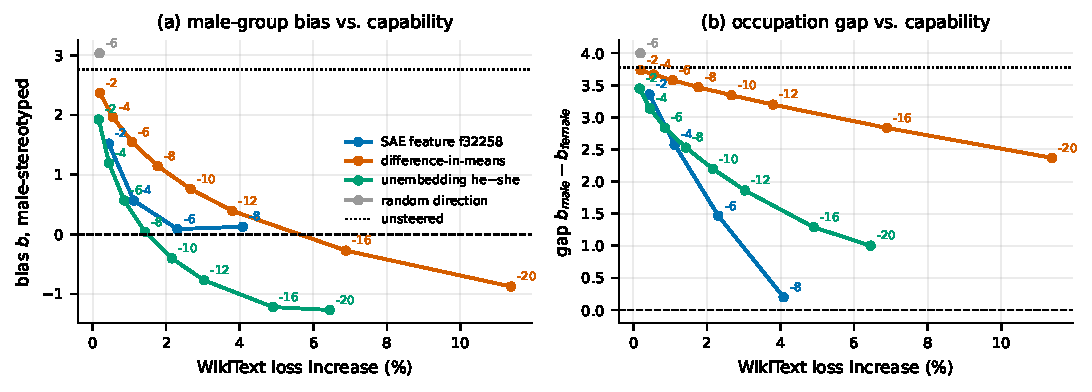
\includegraphics[width=\textwidth]{figures/fig_frontier.pdf}
\caption{Two frontiers at matched $L_2$ norm; each point is one steering strength, and
lower-left is better. (a) Bias on male-stereotyped occupations, the metric we first
reported: the unembedding direction wins. (b) The occupation gap $b_{\text{male}} -
b_{\text{female}}$, which is the stereotype itself: only the SAE feature closes it.
Baseline strengths beyond $-8$ were added for this version (Table~\ref{tab:gap}).}
\label{fig:frontier}
\end{figure}
The comparison that decides whether an SAE is doing work is against the cheap
alternative. We compare four directions at identical $L_2$ norm: the SAE decoder
direction, difference-in-means between mean layer-8 final-position activations on male- and
female-stereotyped templates, the raw unembedding direction
$W_U[\text{`` he''}] - W_U[\text{`` she''}]$, and random Gaussian directions. The random
ones are flat ($\Delta b = +0.27$ at $s=-6$), which is what makes the matched-norm
comparison informative rather than a demonstration that any large perturbation moves a bias
metric.

Which direction wins depends on what is scored, and the earlier version of this paper
scored only one thing. On the male-stereotyped group alone (Figure~\ref{fig:frontier}a)
the order is unembedding, SAE feature, difference-in-means, random. The raw unembedding
direction reaches $b=+0.04$ at \DlossUnembed{} WikiText loss where the feature needs
\DlossSAE{}, and it costs two lines of code. But a direction can win that metric by moving
\emph{every} occupation toward `` she''. The stereotype is the occupation dependence, so we
also score the gap between groups, $b_{\text{male}}-b_{\text{female}}$
(Figure~\ref{fig:frontier}b, Table~\ref{tab:gap}). Here the order reverses. The unsteered
gap is \GapBase{}. At about \DlossSAE{} loss the feature leaves \GapSaeSix{} and the
unembedding direction \GapUnembTen{} (at $s=-10$). The feature closes it to \GapSaeEight{}
\GapSaeEightCI{} at \DlossSAEEight{}. The unembedding direction never does: at $s=-20$, for
\DlossUnembTwenty{}, it leaves \GapUnembTwenty{} \GapUnembTwentyCI{} while pushing the
male-stereotyped group well past parity ($b={}$\BUnembTwentyMale). Below about $1.5\%$ loss
the two are level. On held-out occupations the gap falls from \HeldGapBase{} to
\HeldGapSaeSix{} under the feature and to \HeldGapUnembSix{} under the unembedding
direction at $s=-6$. The gap metric is post hoc: we introduced it for this
version, after the parity results were in.

The SAE direction is not a rediscovery of either alternative (cosine $0.16$ with
difference-in-means, $0.06$ with unembedding). It is also the only one of the three we can
name, from what it responds to in natural text (\S\ref{sec:discovery}). For parity on one
group per unit perplexity, the evidence does not justify an SAE. For removing the
occupation dependence, and knowing what was removed, it does.

\subsection{Three controls}
\label{sec:controls}

\paragraph{Negative control.} \ff{27420} passed selectivity but not output push, and we
kept it to test whether the second criterion earns its place. Across the full sweep it
moves the male-stereotyped log-odds by at most $0.01$ against $2.68$ for \ff{32258}, a
factor of roughly $270$, and its largest female-group shift is $\Delta b = -0.12$
against $3.63$. It also illustrates the caution of \S\ref{sec:setup}: that $-0.12$ sits
at the $p$ floor, because a negligible shift is perfectly consistent across 12
occupations in a deterministic model. A study reporting significance without effect size
would call this feature causal. Had we steered only selectivity-passing candidates, we
would have reported a null result.

\paragraph{Position.} Adding the direction at every position leaves open a less
interesting reading: that we injected a global he-prior instead of changing how the
occupation is represented. Restricting the intervention to the final token settles it. At
$s=-6$ the male-stereotyped log-odds stay at $+2.37$, against $+2.76$ unsteered and $+0.09$
when every position is steered; steering everything except the final token recovers most of
the effect ($+0.68$). The work is done where the occupation is read, not where the pronoun
is predicted.

\paragraph{Layer, readout, prompting.} The direction is not unique to layer 8 but it is
confined to mid-network: injected at layers 4, 6, 8 and 10 it brings the male-stereotyped
group to $+0.55$, $+0.36$, $+0.09$ and $-0.08$, while at layers 12 and 14 it does almost
nothing ($+2.04$, $+2.57$; Table~\ref{tab:layer}). Two caveats on the readout, both in
Appendix~\ref{app:specificity} (Tables~\ref{tab:position}--\ref{tab:prompting} and
Figure~\ref{fig:specificity}). The pronouns carry only $15$--$28\%$ of the next-token mass
and the argmax is usually `` the'' (Table~\ref{tab:readout}), so $b$ measures a contrast
between two candidates rather than the model's single most likely continuation. And prompting is a real but
partial alternative: an instruction to avoid gendered assumptions moves the
male-stereotyped group from $+2.76$ to $+1.61$, and an instruction to use singular
\emph{they} to $+2.12$. Neither reaches the parity that steering and projection do.

\subsection{Necessity: what survives projecting the direction out}
\label{sec:ablation}

Steering tests sufficiency; removal tests necessity. We replace the layer-8 residual $x$
by $x - (x\cdot\hat d)\hat d$ at every position and ask whether the stereotype survives
(Table~\ref{tab:ablation}). Most of it does not. On the discovery templates the
male-stereotyped log-odds fall from \BaseMale{} to \ProjTpl{} \ProjTplCI{}, and on the
held-out occupations from \HeldBase{} to \ProjHeld{} \ProjHeldCI{}, slightly past parity, at
$+2.6\%$ WikiText loss. Projecting out difference-in-means instead leaves far more
behind ($+2.76 \to +1.27$). So on these probes the direction is close to necessary, not
merely sufficient, which is a stronger claim than steering alone can support and the
reason we ran the test.

Two things keep this from being a clean mitigation result. Projection also pushes the
female-stereotyped group further toward `` she'' ($-1.02 \to -1.75$), so it is not a
symmetric debiasing operation. It removes a masculine-referent component wherever that
component is present, which is what \S\ref{sec:discovery} says the feature is. The
capability cost is also comparable to steering, so removal is not the cheaper route. What
the test does establish is that the SAE picked out a direction the behaviour depends on,
not one of several redundant handles.

\subsection{Context override, and capability cost}
\label{sec:override}

At baseline the model respects explicit evidence: given ``The mechanic tied \textbf{her}
hair back before'' it prefers `` she''. Whether amplifying the feature can override a
pronoun the model has already read is the most striking claim available here, and our
earlier version used 4 prompts per side, which is not merely imprecise but untestable:
with $n=4$ a two-sided signed-rank test cannot return $p<0.125$ at any effect size. We rebuilt it at 12
counter-stereotypical prompts per side (Table~\ref{tab:override}). The feature does override
the text, with a sharp crossover: given an explicit `` her'', the model prefers `` she'' in
at least $11$ of $12$ cases up to $s=+3$, splits $6/12$ at $s=+4$, and prefers `` he'' in
$12/12$ by $s=+6$ ($b$: $-3.05 \to +1.16$). The mirror case never occurs, as a masculine-referent
feature predicts: with an explicit `` his'' the stereotype wins at no strength, because
steering never argues for `` she''.

Capability is measured as WikiText next-token loss on held-out passages
(Table~\ref{tab:baselines}). A 10-item factual QA check is reported there for completeness
only, because at $n=10$ a one-item difference is noise. At the strengths that reach
male-group parity, WikiText loss rises by a few percent.

\subsection{More occupations, and generated text}
\label{sec:beyond}

Two limits of the evaluation above are its 12 occupations per group, and a metric that
reads two tokens carrying only 15--28\% of next-token mass. We added an expanded
probe set and a generation-level evaluation. One caveat applies to both. The SAE checkpoint
is distributed through a third-party catalog that was unreachable when we prepared this
version, so these evaluations cover the unsteered model and the two matched-norm baselines,
whose directions need no SAE. Before computing anything new we required every condition to
reproduce its saved value from the original runs (largest relative error
$\ReproMaxErr$). The released code runs the SAE conditions whenever the checkpoint is
present.

\paragraph{Expanded probes.} We used the 40 WinoBias occupations \citep{zhao2018}, split
male/female by US labour statistics, under \XFrames{} frames, with the occupation as the
unit of analysis ($n=\XNMale$ per group, \XOverlap{} shared with discovery;
Table~\ref{tab:expanded}). The male-side stereotype replicates: $b={}$\XBaseMale{}
\XBaseMaleCI{}, against \BaseMale{} on discovery. The female side does not mirror it. The
20 female-majority occupations average \XBaseFemale{} \XBaseFemaleCI{}, and only a few
(nurse, housekeeper, receptionist, hairdresser) lean strongly toward `` she''. On next-token
evidence the model has one broad masculine default rather than two symmetric stereotypes,
as the masculine-referent reading of \S\ref{sec:discovery} predicts.

\paragraph{Generated text.} For \GenNOcc{} occupations per group (WinoBias plus held-out)
we sampled continuations of 40--60 tokens at temperature 0.7, in raw completion and under
the chat template, and scored the first third-person pronoun the model wrote
(Table~\ref{tab:generation}; \GenNPerCond{} generations per condition). This is a proxy,
since the first pronoun occasionally refers to another character. Two findings bear on the
metric. Next-token $b$ orders occupations almost exactly as generation does (Spearman
$\rho={}$\ValidRawRho{} raw, \ValidChatRho{} chat, over the 40 WinoBias occupations), so it is
a valid \emph{ordinal} measure. Its zero point is not reliable: in generation the
female-stereotyped group is strongly stereotyped (only \GenRawFemBase{} of its gendered
first pronouns are `` he'' in raw completion and \GenChatFemBase{} under the chat
template), which a next-token mean near zero hides. The same offset matters for
interventions. A strength that reaches next-token parity overshoots in free text: the
unembedding direction at $s=-6$ takes the male group's he-share from \GenRawBase{} to
\GenRawUnembSix{}, and to \GenRawUnembEight{} at $s=-8$, past the 50\% mark. Meanwhile it
drives the female group's he-share from \GenRawFemBase{} to \GenRawFemUnembSix{},
with fluency unchanged. The between-group gap shrinks (\GenRawGapBase{} to
\GenRawGapUnembSix{} percentage points), partly because a share cannot fall below zero.
What the direction produces is a uniform `` she'' default, not the absence of an
occupation prior.

\section{Cross-model comparison, and a correction}
\label{sec:crossmodel}

We ran the pipeline on LFM2.5-230M at both layers with public SAEs (9 and 5), then ran the
same two-sided search in Llama. That second step caught the error below. The bias runs the same way in LFM2.5 and is weaker: $b={}$\LfmBaseMale{} \LfmBaseMaleCI{} on
male-stereotyped occupations against Llama's \BaseMale{}, with female-stereotyped at \LfmBaseFemale{}.
The smaller, less heavily instruction-tuned model is the less biased.

\paragraph{What we first concluded, and what was wrong with it.}
In LFM2.5 the top-ranked masculine candidate (\ff{12288}) does almost nothing: a log-odds
swing of $+0.29$ across $s\in[-6,+6]$. The top-ranked feminine candidate, \ff{9619}, does a
great deal: $-6.49$ on male-stereotyped and $-7.56$ on female-stereotyped prompts, enough
that at $s=+6$ even male-stereotyped occupations become `` she''-preferring. In Llama the
pattern is the reverse. Read off rank~1 alone, the models look like mirror images, which
is what we originally reported. Searching deeper says otherwise. LFM2.5 does have a masculine handle: \ff{17579} at rank~2
swings the male-stereotyped group by $+3.16$ and \ff{32504} at rank~5 by $+2.24$
(Table~\ref{tab:searchfull}). Our score simply did not put it first.

\paragraph{What survives, once both models are searched to depth 5.}
The asymmetry is real, but it is not a mirror image. In Llama the masculine handle is
rank~1 and strong ($+4.05$) while ranks 2--5 are inert ($\le +0.52$), and \emph{nothing} on
the feminine side moves the behaviour (best swing $-0.67$). In LFM2.5 both polarities have
a handle, and the feminine one is about twice as strong as the masculine one ($6.49$ against
$3.16$). So Llama exposes one steerable polarity and LFM2.5 exposes two, unevenly. A recipe
of the form ``clamp the top-scoring feature of this polarity'' therefore lands very
differently in the two models, but not because either model lacks the mechanism.

Rank is a weak predictor of causal effect: the rank-1 candidate is the strongest handle in
two of the four (model, polarity) cells and inert in a third, so a null reported from a
single candidate, as ours was, is not evidence of absence. The handle is also layer-specific. At LFM2.5's layer 5 nothing on either side
moves the male-stereotyped group by more than $1.11$ log-odds, against $6.49$ at layer 9.

\section{Related work}
\label{sec:related}

Behavioural work on gender bias runs from static embeddings
\citep{bolukbasi2016,caliskan2017} through the coreference benchmarks
\citep{rudinger2018,zhao2018}, from which we take occupation stereotype assignments but not
their coreference structure. On the interpretability side, \citet{bricken2023} established
dictionary learning on LM residuals and \citet{templeton2024} scaled it with feature
steering; \citet{lieberum2024} is the reference open SAE release, and its documentation of
input normalisation is the direct context for \S\ref{sec:preflight}. For steering we follow
the activation-addition line \citep{turner2023,rimsky2024,li2023}, in particular the sweep
protocol of \citet{rimsky2024}, whose contrastive construction is also our
difference-in-means baseline. Our output-push test is a single-feature form of direct logit
attribution, in the tradition of the logit lens \citep{nostalgebraist2020,belrose2023}.
Closest to this paper, \citet{vig2020} attributed gender bias to specific neurons by causal
mediation, and \citet{marks2024} introduced SHIFT, ablating SAE features that carry
unintended signal from a classifier: more rigorous than \S\ref{sec:dose} on circuit-level
attribution, but applied to a classifier rather than open-ended generation.

\section{Limitations}
\label{sec:limitations}

Two models is an existence proof, not a distribution, and we make no claim about how often
anything we saw occurs. Discovery ran at one layer per model because that is what public
SAE coverage allowed, and the layer-5 result in \S\ref{sec:crossmodel} shows the choice is
not free, so a full layer scan is the most valuable extension. The SAE's operating point is
imperfect at $L_0\approx3.6$k where hundreds would be expected, which limits what we can
claim about \ff{32258} being monosemantic, though not the causal results. Our search stops
at depth 5 in Llama and 8 in LFM2.5, so there may be handles we did not reach.

The evaluation is narrow in ways this version only partly fixes. It covers one bias axis,
and a binary one: `` he'' against `` she'', with `` they'' measured only as a secondary
quantity. Non-binary pronouns deserve to be a first-class axis, and grammatical gender in
other languages is untouched. The expanded probes (20 occupations per group, labelled from
labour statistics) and the generation evaluation of \S\ref{sec:beyond} cover the unsteered
model and the two baselines, but not the SAE feature, whose checkpoint was unavailable to
us. For \ff{32258} itself the evidence therefore remains 12
occupations per group plus the 24 held-out ones, read at the next token. Generations are
short (40--60 tokens) and scored by their first pronoun, so consistency over a long
narrative is untested. The main results query an instruction-tuned model in raw completion
format; the chat-template generations agree in direction but are not a deployment study.

\section{Broader impact}

We report how to amplify a stereotype as well as reduce it, including a strength at which the
model contradicts a pronoun it has read; the misuse risk is narrow, since the intervention
needs white-box access. The mitigation direction deserves more caution: these results do not
endorse feature clamping for deployment. A system that closes the pronoun gap on probes like
ours while keeping the representation that produced it would be worse than an honest biased
one, because the measurement would no longer reveal the problem.

\section{Conclusion}

A single SAE feature in Llama-3.2-1B-Instruct is a working, nearly necessary handle on
occupation$\rightarrow$pronoun stereotyping, and verification changed three things we
would otherwise have published: which baseline wins depended on scoring one group's parity
or the occupation gap, a top-ranked discovery candidate was inert, and a cross-model claim
drawn from rank~1 did not survive a deeper search. The lesson is procedural, and
Appendix~\ref{app:checklist} collects it as a checklist.

{\small
\bibliographystyle{plainnat}
\bibliography{refs}
}

\appendix

\section{Probe sets}\label{app:probes}

All prompts end immediately before a pronoun. Stereotype assignments follow
\citet{zhao2018} and \citet{rudinger2018}.

\paragraph{Discovery (36 matched templates), ``The \{occupation\} said that''.}
\emph{Male-stereotyped:} mechanic, engineer, pilot, plumber, electrician, carpenter, truck
driver, firefighter, surgeon, programmer, security guard, construction worker.
\emph{Female-stereotyped:} nurse, receptionist, secretary, librarian, babysitter,
housekeeper, hairdresser, florist, dietitian, social worker, kindergarten teacher, flight
attendant. \emph{Neutral:} person, employee, neighbor, customer, student, colleague,
stranger, visitor, worker, adult, individual, citizen.

\paragraph{Varied predicate (24).} The same occupations under different frames, e.g.\
``The mechanic finished the repair and then''. This varies the frame but \emph{not} the
occupations, which is why the next set exists.

\paragraph{Held out (48 prompts, 24 occupations).} Occupations appearing nowhere in
discovery, under two template families also appearing nowhere in discovery (``The
\{occupation\} explained that''; ``After the shift ended, the \{occupation\} admitted
that''). \emph{Male-stereotyped:} welder, machinist, roofer, bricklayer, miner, butcher,
crane operator, logger, sheet metal worker, mover, boilermaker, millwright.
\emph{Female-stereotyped:} midwife, nanny, seamstress, dental hygienist, manicurist,
paralegal, preschool teacher, speech therapist, dressmaker, home health aide, occupational
therapist, dance teacher.

\paragraph{Context override (24).} Counter-stereotypical prompts containing an explicit
pronoun: 12 male-stereotyped occupations with a female-marking clause (``The mechanic tied
\textbf{her} hair back before'') and 12 female-stereotyped occupations with a male-marking
clause (``The nurse adjusted \textbf{his} stethoscope and then'').

\section{Three discovery attempts that failed}\label{app:failures}

\paragraph{Attempt 1: contrast male- against female-occupation prompt sets.} Top candidate
\ff{3432}, about $1\%$ difference on large baseline activations; its decoder direction
projects onto no interpretable tokens. \emph{Why it fails:} the sets differ in subject
matter as well as implied gender, repairs and wiring versus patients and phones, and the
largest activation differences track the largest differences, which are topical. The
matched-template design exists to remove this, and \ff{9392} (food) is its residue even
after matching.

\paragraph{Attempt 2: bucket by the model's own pronoun choice.} Neutral ``Continue this
story\dots'' prompts, bucketed by whether the model produced `` he'' or `` she''.
Differences around $0.5\%$. \emph{Why it fails:} activations were mean-pooled over all
positions, while the signal lives at the final position; pooling over ten or more
positions buries it.

\paragraph{Attempt 3: per-prompt tracing.} Eight probes traced individually, collecting
features that peak at pronoun positions. Surfaced \ff{26265}, which fires on both ``his''
and ``her'', which is possession rather than stereotype, and also \ff{2546} and
\ff{32258}. \emph{Why
it fails alone:} eight prompts and a top-$k$ cutoff cannot rank candidates. \emph{Why it
was still worth doing:} \ff{32258} was later found independently by the systematic method,
and two unrelated techniques agreeing was the first real evidence we had.

\begin{table}[h]
\centering
\caption{Candidates. Activation is the mean at the final position over 12 matched
templates per group; ``push'' is the he$-$she logit difference induced by the decoder
direction at unit activation; density is the fraction of held-out WikiText positions
where the feature is active. Characterisations come from max-activating contexts and
vocabulary projections (Appendix~\ref{app:feature}).}
\label{tab:candidates}
\small
\begin{tabular}{lrrrrrl}
\toprule
& \multicolumn{3}{c}{activation} & & density & \\
\cmidrule(lr){2-4}
feature & male & female & neutral & push & (\%) & what it turns out to be \\
\midrule
\ff{32258} & 0.38 & 0.03 & 0.16 & $+0.017$ & 15.9 & masculine-referent context \\
\ff{27420} & 0.11 & 0.29 & 0.00 & $-0.011$ & 14.0 & low-magnitude, no coherent theme \\
\ff{9392} & 0.32 & 0.73 & 0.24 & $+0.006$ & 16.8 & food (fires on \emph{dietitian}) \\
\ff{26265} & 0.00 & 0.00 & 0.00 & $+0.002$ & 10.6 & possessive determiner \\
\bottomrule
\end{tabular}
\end{table}

\begin{figure}[h]
\centering
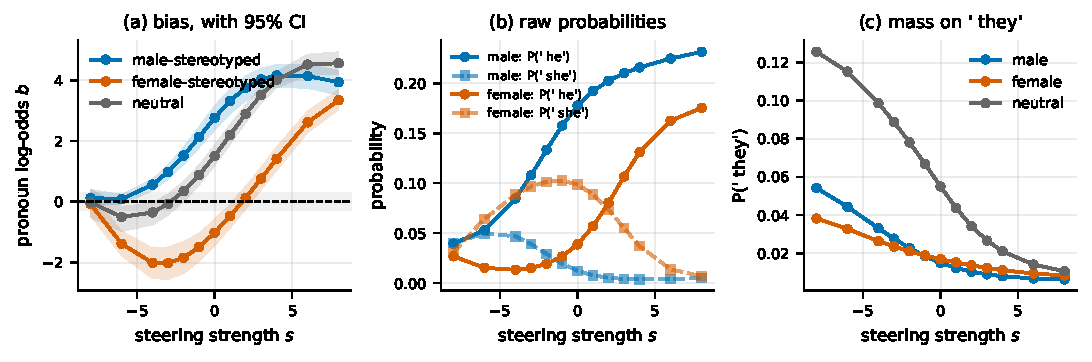
\includegraphics[width=\textwidth]{figures/fig_dose_ci.pdf}
\caption{Dose--response for \ff{32258} with $95\%$ bootstrap CIs over occupations.
(a) pronoun log-odds; the shaded band is parity. (b) raw probabilities, for comparability
with ratio-style reporting. (c) mass on `` they'', which \emph{rises} under debiasing.}
\label{fig:dose}
\end{figure}
\section{Feature characterisation}\label{app:feature}

Measured on 100 held-out WikiText passages, excluding the first positions of each
(\S\ref{sec:preflight}).

\paragraph{\ff{32258}.} Density $15.9\%$. Promotes `` himself'', `` his'', ``his'',
``His'', `` Himself'', and masculine possessives in other languages. Maximally activating
contexts have an established male referent: ``\dots{}role on the television series The
Bill ; he'', ``\dots{}at WJR radio in Detroit , but he'', ``In college , he'', ``The tenor
of his''. Nearest decoder neighbours by cosine: \ff{8980} $(0.41)$, \ff{6365} $(0.35)$,
\ff{19041} $(0.30)$, so not an isolated direction, which is relevant to
\S\ref{sec:ablation}.

\paragraph{\ff{9392} (rejected: topic).} Density $16.8\%$. Promotes `` food'', `` foods'',
`` meal'', `` nutritional'', `` recipe''. Fires more on the female-stereotyped set
($0.73$) than the male one ($0.32$) because \emph{dietitian} is in it. Ranked first by
selectivity alone.

\paragraph{\ff{26265} (rejected: grammatical).} Density $10.6\%$. Promotes `` own'',
``self'', `` respective''. Maximally activating contexts: ``took his'', ``making their'',
``adapted to his'', ``turned its'', ``bar their''. Activation on all three template sets
is $\approx 0$, because those templates contain no possessive.

\paragraph{\ff{27420} (negative control).} Density $14.0\%$. Promotes `` tonight'',
`` security'', `` guards'' and `` ward'', with no coherent theme. Away from the anomalous early
positions its activations stay below $1.0$ throughout the WikiText sample, the most likely
reason steering it does nothing: there is little for the direction to add.

\begin{figure}[h]
\centering
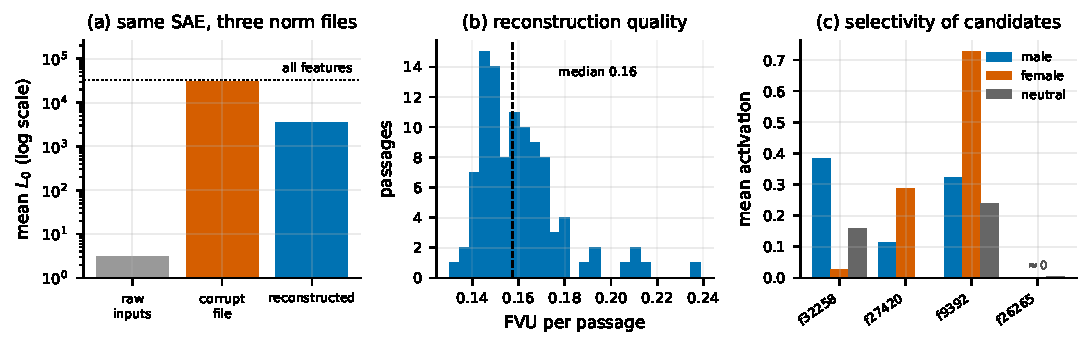
\includegraphics[width=\textwidth]{figures/fig_preflight.pdf}
\caption{(a) Mean $L_0$ under the three normalisation states, log scale. (b) Per-passage
FVU with the reconstructed statistics, spanning $0.130$ to $0.239$ across 100 passages
(mean $0.160$, median $0.157$). (c) Selectivity of the four candidate features on the
matched template sets.}
\label{fig:preflight}
\end{figure}

\section{Logit lens and layer ablation}\label{app:trace}

For a representative biased completion, the logit lens shows early layers copying the
final prompt token, with the pronoun prediction resolving only in the upper layers, and
single-layer ablation shows the prediction depends on layers 9--14, immediately
downstream of the layer-8 read point. Two consequences: reading at layer 8 catches the
stereotype before the prediction is committed, and the steering effect must be mediated by
those downstream layers rather than by the direct path to the unembedding
(\S\ref{sec:discovery}).

\section{Specificity controls}\label{app:specificity}

Four controls that decide what the main result means rather than whether it holds:
which token positions carry the effect (Table~\ref{tab:position}), whether layer 8 is
special (Table~\ref{tab:layer}), how much probability the pronouns actually carry
(Table~\ref{tab:readout}), and whether an instruction achieves the same thing more
cheaply (Table~\ref{tab:prompting}). Figure~\ref{fig:specificity} plots the first, second
and fourth.

\begin{table}[h]
\centering
\caption{Position decomposition of the intervention, pronoun log-odds $b$. Steering the
final token alone leaves the male-stereotyped group at $+2.37$, against $+2.76$ unsteered,
so the effect is not a readout-time prior. It is carried by the earlier positions, where
the occupation is read.}
\label{tab:position}
\small
\begin{tabular}{lcccc}
\toprule
& \multicolumn{2}{c}{$s=-6$} & \multicolumn{2}{c}{$s=+6$} \\
\cmidrule(lr){2-3}\cmidrule(lr){4-5}
positions steered & male-stereo & female-stereo & male-stereo & female-stereo \\
\midrule
all positions & $+0.09$ & $-1.38$ & $+4.14$ & $+2.61$ \\
final position only & $+2.37$ & $-1.26$ & $+3.14$ & $+0.14$ \\
all but final & $+0.68$ & $-1.19$ & $+4.23$ & $+1.79$ \\
\midrule
unsteered & \multicolumn{4}{c}{male $+2.76$, female $-1.02$} \\
\bottomrule
\end{tabular}
\end{table}

\begin{table}[h]
\centering
\caption{Injecting $d_{32258}$ at other layers, pronoun log-odds $b$. The direction was
derived from the layer-8 SAE.}
\label{tab:layer}
\small
\begin{tabular}{lcccc}
\toprule
& \multicolumn{2}{c}{$s=-6$} & \multicolumn{2}{c}{$s=+6$} \\
\cmidrule(lr){2-3}\cmidrule(lr){4-5}
injection layer & male-stereo & female-stereo & male-stereo & female-stereo \\
\midrule
2 & $+1.08$ & $-0.49$ & $+1.35$ & $+2.98$ \\
4 & $+0.55$ & $-1.31$ & $+3.89$ & $+2.51$ \\
6 & $+0.36$ & $-1.74$ & $+4.05$ & $+2.48$ \\
8 & $+0.09$ & $-1.38$ & $+4.14$ & $+2.61$ \\
10 & $-0.08$ & $-5.31$ & $+5.30$ & $+1.23$ \\
12 & $+2.04$ & $-2.21$ & $+3.50$ & $-0.23$ \\
14 & $+2.57$ & $-1.16$ & $+2.99$ & $-0.87$ \\
\bottomrule
\end{tabular}
\end{table}

\begin{table}[h]
\centering
\caption{Readout diagnostics at baseline: how much probability the pronouns actually
carry. Ranks are medians over 12 prompts per group.}
\label{tab:readout}
\small
\begin{tabular}{lrrrl}
\toprule
group & pronoun mass & rank `` he'' & rank `` she'' & most common top-1 tokens \\
\midrule
male-stereo & 0.205 & 2 & 12 & ``the'' (10), ``he'' (2) \\
female-stereo & 0.154 & 5 & 2 & ``the'' (12) \\
neutral & 0.277 & 2 & 4 & ``the'' (8), ``he'' (4) \\
\bottomrule
\end{tabular}
\end{table}

\begin{table}[h]
\centering
\caption{Prompting baseline: pronoun log-odds $b$ with $95\%$ CI, prefixes prepended to
the same probes.}
\label{tab:prompting}
\footnotesize
\setlength{\tabcolsep}{4pt}
\begin{tabular}{llll}
\toprule
prefix & male-stereo & female-stereo & neutral \\
\midrule
no instruction & $+2.76$ $[+2.35,+3.15]$ & $-1.02$ $[-1.45,-0.59]$ & $+1.51$ $[+1.18,+1.87]$ \\
gender-neutral instruction & $+1.61$ $[+1.19,+2.01]$ & $-1.45$ $[-1.81,-1.12]$ & $+0.33$ $[-0.05,+0.71]$ \\
explicit ``use they'' instruction & $+2.12$ $[+1.58,+2.60]$ & $-1.86$ $[-2.34,-1.39]$ & $+0.70$ $[+0.29,+1.11]$ \\
\bottomrule
\end{tabular}
\end{table}

\begin{figure}[h]
\centering
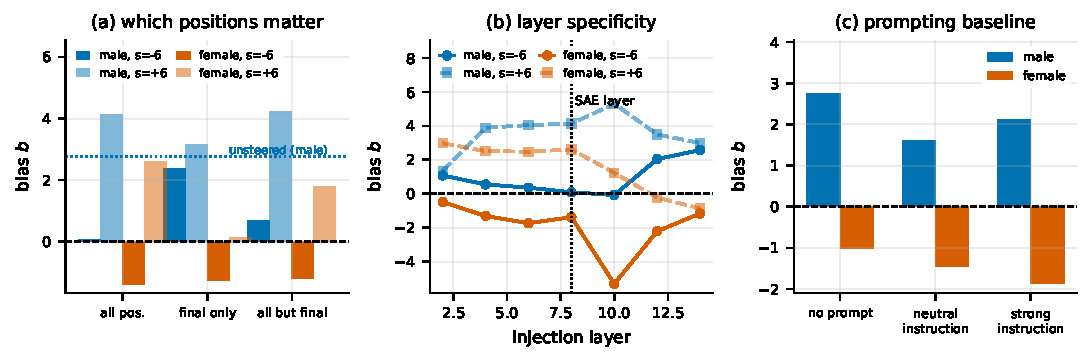
\includegraphics[width=\textwidth]{figures/fig_specificity.pdf}
\caption{(a) Position decomposition. (b) Layer specificity; the dotted line marks the
SAE's own layer. (c) Prompting baseline.}
\label{fig:specificity}
\end{figure}

\section{Full tables}\label{app:fulltables}

The tables behind the summary numbers in the main text: capability against bias at the
debiasing strengths (Table~\ref{tab:baselines}) and across every measured strength
(Table~\ref{tab:baselinesfull}), the necessity test (Table~\ref{tab:ablation}), the full
dose--response sweep (Table~\ref{tab:dosefull}), transfer to unseen occupations
(Table~\ref{tab:heldout}), the context-override sweep (Table~\ref{tab:override}), and the
two-sided feature search in both models at every layer we could reach
(Table~\ref{tab:searchfull}), and the later additions: generation
(Table~\ref{tab:generation}), expanded probes (Table~\ref{tab:expanded}) and the
occupation gap (Table~\ref{tab:gap}).

\begin{table}[h]
\centering
\caption{Bias and capability at matched intervention norm, male-stereotyped group.
Shown at the debiasing strengths; the full sweep is Table~\ref{tab:baselinesfull}.
$\Delta$loss is the change in WikiText next-token loss against the unsteered model. QA is
10 factual items, reported for completeness only: at $n=10$ a one-item difference is not
evidence and we draw no conclusion from it.}
\label{tab:baselines}
\small
\begin{tabular}{llllrrr}
\toprule
direction & $s$ & $b$ [95\% CI] & $\Delta b$ & loss & $\Delta$loss & QA \\
\midrule
unsteered & --- & $+2.76$ $[+2.36,+3.15]$ & --- & 3.270 & --- & 10/10 \\
\midrule
SAE feature \ff{32258} & $-8$ & $+0.13$ $[-0.12,+0.40]$ & $-2.64$ & 3.404 & $+4.1\%$ & --- \\
 & $-6$ & $+0.09$ $[-0.07,+0.24]$ & $-2.68$ & 3.346 & $+2.3\%$ & 9/10 \\
\midrule
difference-in-means & $-8$ & $+1.14$ $[+0.86,+1.42]$ & $-1.62$ & 3.328 & $+1.8\%$ & 9/10 \\
 & $-6$ & $+1.55$ $[+1.23,+1.86]$ & $-1.21$ & 3.305 & $+1.1\%$ & --- \\
\midrule
unembedding he$-$she & $-8$ & $+0.04$ $[-0.18,+0.28]$ & $-2.72$ & 3.317 & $+1.4\%$ & --- \\
 & $-6$ & $+0.57$ $[+0.32,+0.82]$ & $-2.19$ & 3.298 & $+0.9\%$ & 10/10 \\
\midrule
random direction & $-6$ & $+3.03$ $[+2.60,+3.47]$ & $+0.27$ & 3.276 & $+0.2\%$ & --- \\
\bottomrule
\end{tabular}
\end{table}
\begin{table}[h]
\centering
\caption{Necessity test: projecting the direction out of the layer-8 residual at every
position, $x \mapsto x - (x\cdot\hat d)\hat d$, rather than adding it. $\Delta b$ is
paired against the unmodified model on the male-stereotyped group.}
\label{tab:ablation}
\scriptsize
\setlength{\tabcolsep}{3pt}
\begin{tabular}{lllll}
\toprule
probe set & intervention & $b$ male-stereo & $b$ female-stereo & $\Delta b$ (male) \\
\midrule
discovery templates & unmodified & $+2.76$ $[+2.36,+3.15]$ & $-1.02$ $[-1.45,-0.58]$ & --- \\
 & project out \ff{32258} & $+0.27$ $[+0.11,+0.43]$ & $-1.75$ $[-2.27,-1.26]$ & $-2.49$ ($\le$4.9e-4) \\
 & project out difference-in-means & $+1.27$ $[+0.93,+1.59]$ & $-1.01$ $[-1.38,-0.64]$ & $-1.49$ ($\le$4.9e-4) \\
\midrule
held-out occupations & unmodified & $+2.52$ $[+2.30,+2.74]$ & $-1.81$ $[-2.19,-1.45]$ & --- \\
 & project out \ff{32258} & $-0.20$ $[-0.38,-0.02]$ & $-2.82$ $[-3.24,-2.42]$ & $-2.73$ ($\le$4.9e-4) \\
 & project out difference-in-means & $+0.82$ $[+0.61,+1.05]$ & $-2.39$ $[-2.86,-1.96]$ & $-1.70$ ($\le$4.9e-4) \\
\bottomrule
\end{tabular}
\end{table}

\begin{table}[h]
\centering
\caption{Full dose--response sweep for \ff{32258}: every strength and all three groups.
The main text quotes $s=+4$ and $s=\pm8$ from this table.}
\label{tab:dosefull}
\scriptsize
\setlength{\tabcolsep}{3pt}
\begin{tabular}{lrrrrllrr}
\toprule
group & $s$ & $\phe$ & $\pshe$ & $\pthey$ & $b$ [95\% CI] & $\Delta b$ [95\% CI] & $p$ & $d_z$ \\
\midrule
male-stereo & $+0$ & 0.178 & 0.012 & 0.0149 & $+2.76$ $[+2.36,+3.14]$ & --- & --- & --- \\
 & $-8$ & 0.039 & 0.040 & 0.0542 & $+0.13$ $[-0.12,+0.41]$ & $-2.64$ $[-3.15,-2.07]$ & $\le$4.9e-4 & $-2.60$ \\
 & $-6$ & 0.053 & 0.050 & 0.0443 & $+0.09$ $[-0.07,+0.25]$ & $-2.68$ $[-3.08,-2.26]$ & $\le$4.9e-4 & $-3.48$ \\
 & $-4$ & 0.085 & 0.047 & 0.0331 & $+0.56$ $[+0.37,+0.75]$ & $-2.20$ $[-2.49,-1.91]$ & $\le$4.9e-4 & $-4.05$ \\
 & $-3$ & 0.108 & 0.039 & 0.0276 & $+0.99$ $[+0.75,+1.21]$ & $-1.78$ $[-2.00,-1.55]$ & $\le$4.9e-4 & $-4.23$ \\
 & $-2$ & 0.133 & 0.029 & 0.0227 & $+1.52$ $[+1.22,+1.80]$ & $-1.24$ $[-1.40,-1.09]$ & $\le$4.9e-4 & $-4.38$ \\
 & $-1$ & 0.158 & 0.019 & 0.0184 & $+2.13$ $[+1.78,+2.47]$ & $-0.63$ $[-0.71,-0.56]$ & $\le$4.9e-4 & $-4.57$ \\
 & $+1$ & 0.192 & 0.008 & 0.0122 & $+3.32$ $[+2.90,+3.72]$ & $+0.56$ $[+0.50,+0.63]$ & $\le$4.9e-4 & $+4.68$ \\
 & $+2$ & 0.203 & 0.005 & 0.0103 & $+3.75$ $[+3.33,+4.15]$ & $+0.99$ $[+0.86,+1.12]$ & $\le$4.9e-4 & $+4.11$ \\
 & $+3$ & 0.210 & 0.004 & 0.0089 & $+4.02$ $[+3.62,+4.40]$ & $+1.26$ $[+1.07,+1.47]$ & $\le$4.9e-4 & $+3.36$ \\
 & $+4$ & 0.216 & 0.004 & 0.0079 & $+4.16$ $[+3.76,+4.53]$ & $+1.40$ $[+1.13,+1.68]$ & $\le$4.9e-4 & $+2.74$ \\
 & $+6$ & 0.225 & 0.004 & 0.0067 & $+4.14$ $[+3.73,+4.52]$ & $+1.37$ $[+1.03,+1.78]$ & $\le$4.9e-4 & $+1.97$ \\
 & $+8$ & 0.231 & 0.005 & 0.0063 & $+3.93$ $[+3.51,+4.33]$ & $+1.17$ $[+0.79,+1.62]$ & $\le$4.9e-4 & $+1.53$ \\
\midrule
female-stereo & $+0$ & 0.039 & 0.099 & 0.0169 & $-1.02$ $[-1.46,-0.59]$ & --- & --- & --- \\
 & $-8$ & 0.027 & 0.031 & 0.0382 & $-0.07$ $[-0.47,+0.32]$ & $+0.95$ $[+0.31,+1.61]$ & 2.7e-2 & $+0.78$ \\
 & $-6$ & 0.015 & 0.064 & 0.0327 & $-1.38$ $[-1.77,-0.97]$ & $-0.36$ $[-0.75,+0.03]$ & n.s. & $-0.50$ \\
 & $-4$ & 0.013 & 0.089 & 0.0263 & $-2.01$ $[-2.53,-1.51]$ & $-0.99$ $[-1.23,-0.74]$ & $\le$4.9e-4 & $-2.21$ \\
 & $-3$ & 0.015 & 0.097 & 0.0235 & $-2.02$ $[-2.56,-1.51]$ & $-1.00$ $[-1.20,-0.81]$ & $\le$4.9e-4 & $-2.77$ \\
 & $-2$ & 0.019 & 0.101 & 0.0210 & $-1.84$ $[-2.37,-1.33]$ & $-0.82$ $[-0.96,-0.69]$ & $\le$4.9e-4 & $-3.19$ \\
 & $-1$ & 0.027 & 0.102 & 0.0188 & $-1.49$ $[-1.98,-1.02]$ & $-0.47$ $[-0.55,-0.41]$ & $\le$4.9e-4 & $-3.59$ \\
 & $+1$ & 0.057 & 0.089 & 0.0151 & $-0.47$ $[-0.87,-0.07]$ & $+0.55$ $[+0.49,+0.61]$ & $\le$4.9e-4 & $+4.95$ \\
 & $+2$ & 0.080 & 0.073 & 0.0136 & $+0.13$ $[-0.26,+0.51]$ & $+1.15$ $[+1.05,+1.25]$ & $\le$4.9e-4 & $+5.93$ \\
 & $+3$ & 0.107 & 0.055 & 0.0122 & $+0.76$ $[+0.37,+1.15]$ & $+1.78$ $[+1.64,+1.93]$ & $\le$4.9e-4 & $+6.56$ \\
 & $+4$ & 0.131 & 0.037 & 0.0111 & $+1.41$ $[+1.02,+1.81]$ & $+2.43$ $[+2.24,+2.64]$ & $\le$4.9e-4 & $+6.56$ \\
 & $+6$ & 0.163 & 0.014 & 0.0093 & $+2.61$ $[+2.28,+2.97]$ & $+3.63$ $[+3.28,+4.00]$ & $\le$4.9e-4 & $+5.41$ \\
 & $+8$ & 0.175 & 0.007 & 0.0083 & $+3.34$ $[+3.03,+3.69]$ & $+4.36$ $[+3.82,+4.92]$ & $\le$4.9e-4 & $+4.26$ \\
\midrule
neutral & $+0$ & 0.178 & 0.044 & 0.0550 & $+1.51$ $[+1.18,+1.85]$ & --- & --- & --- \\
 & $-8$ & 0.044 & 0.037 & 0.1256 & $-0.02$ $[-0.51,+0.41]$ & $-1.52$ $[-2.01,-1.02]$ & $\le$4.9e-4 & $-1.67$ \\
 & $-6$ & 0.044 & 0.062 & 0.1153 & $-0.50$ $[-0.97,-0.16]$ & $-2.01$ $[-2.38,-1.64]$ & $\le$4.9e-4 & $-2.95$ \\
 & $-4$ & 0.060 & 0.078 & 0.0987 & $-0.35$ $[-0.77,-0.03]$ & $-1.86$ $[-2.12,-1.62]$ & $\le$4.9e-4 & $-4.01$ \\
 & $-3$ & 0.078 & 0.079 & 0.0888 & $-0.06$ $[-0.44,+0.26]$ & $-1.57$ $[-1.77,-1.39]$ & $\le$4.9e-4 & $-4.56$ \\
 & $-2$ & 0.104 & 0.073 & 0.0781 & $+0.35$ $[+0.01,+0.68]$ & $-1.16$ $[-1.28,-1.04]$ & $\le$4.9e-4 & $-5.09$ \\
 & $-1$ & 0.138 & 0.060 & 0.0667 & $+0.88$ $[+0.55,+1.22]$ & $-0.63$ $[-0.69,-0.57]$ & $\le$4.9e-4 & $-5.37$ \\
 & $+1$ & 0.217 & 0.027 & 0.0437 & $+2.20$ $[+1.87,+2.53]$ & $+0.69$ $[+0.62,+0.77]$ & $\le$4.9e-4 & $+4.92$ \\
 & $+2$ & 0.248 & 0.016 & 0.0341 & $+2.89$ $[+2.59,+3.19]$ & $+1.39$ $[+1.22,+1.56]$ & $\le$4.9e-4 & $+4.37$ \\
 & $+3$ & 0.270 & 0.009 & 0.0266 & $+3.52$ $[+3.24,+3.79]$ & $+2.01$ $[+1.73,+2.30]$ & $\le$4.9e-4 & $+3.84$ \\
 & $+4$ & 0.284 & 0.006 & 0.0210 & $+4.01$ $[+3.74,+4.28]$ & $+2.51$ $[+2.11,+2.90]$ & $\le$4.9e-4 & $+3.42$ \\
 & $+6$ & 0.301 & 0.004 & 0.0140 & $+4.52$ $[+4.19,+4.85]$ & $+3.01$ $[+2.45,+3.56]$ & $\le$4.9e-4 & $+2.91$ \\
 & $+8$ & 0.311 & 0.004 & 0.0105 & $+4.56$ $[+4.19,+4.93]$ & $+3.05$ $[+2.42,+3.66]$ & $\le$4.9e-4 & $+2.65$ \\
\bottomrule
\end{tabular}
\end{table}

\begin{table}[h]
\centering
\caption{Transfer to 24 occupations and two template families appearing nowhere in
discovery, for the SAE direction and both baselines at matched norm.}
\label{tab:heldout}
\small
\begin{tabular}{llllr}
\toprule
group & intervention & $b$ [95\% CI] & $\Delta b$ & $p$ \\
\midrule
male-stereo & unsteered & $+2.52$ $[+2.31,+2.74]$ & --- & --- \\
 & SAE \ff{32258}, $s=-6$ & $-0.53$ $[-0.73,-0.33]$ & $-3.06$ & $\le$4.9e-4 \\
 & SAE \ff{32258}, $s=-3$ & $+0.43$ $[+0.24,+0.61]$ & $-2.10$ & $\le$4.9e-4 \\
 & SAE \ff{32258}, $s=+3$ & $+4.97$ $[+4.74,+5.19]$ & $+2.44$ & $\le$4.9e-4 \\
 & SAE \ff{32258}, $s=+6$ & $+5.61$ $[+5.32,+5.89]$ & $+3.09$ & $\le$4.9e-4 \\
 & difference-in-means, $s=-6$ & $+0.97$ $[+0.78,+1.16]$ & $-1.55$ & $\le$4.9e-4 \\
 & difference-in-means, $s=-3$ & $+1.71$ $[+1.50,+1.92]$ & $-0.81$ & $\le$4.9e-4 \\
 & difference-in-means, $s=+3$ & $+3.37$ $[+3.14,+3.58]$ & $+0.84$ & $\le$4.9e-4 \\
 & difference-in-means, $s=+6$ & $+4.15$ $[+3.95,+4.36]$ & $+1.63$ & $\le$4.9e-4 \\
 & unembedding he$-$she, $s=-6$ & $+0.13$ $[-0.04,+0.30]$ & $-2.40$ & $\le$4.9e-4 \\
 & unembedding he$-$she, $s=-3$ & $+1.14$ $[+0.96,+1.32]$ & $-1.38$ & $\le$4.9e-4 \\
 & unembedding he$-$she, $s=+3$ & $+4.32$ $[+4.08,+4.55]$ & $+1.80$ & $\le$4.9e-4 \\
 & unembedding he$-$she, $s=+6$ & $+6.07$ $[+5.85,+6.28]$ & $+3.55$ & $\le$4.9e-4 \\
\midrule
female-stereo & unsteered & $-1.81$ $[-2.19,-1.45]$ & --- & --- \\
 & SAE \ff{32258}, $s=-6$ & $-2.63$ $[-3.07,-2.19]$ & $-0.81$ & $\le$4.9e-4 \\
 & SAE \ff{32258}, $s=-3$ & $-3.17$ $[-3.61,-2.73]$ & $-1.36$ & $\le$4.9e-4 \\
 & SAE \ff{32258}, $s=+3$ & $+0.28$ $[-0.06,+0.61]$ & $+2.10$ & $\le$4.9e-4 \\
 & SAE \ff{32258}, $s=+6$ & $+2.56$ $[+2.07,+3.06]$ & $+4.38$ & $\le$4.9e-4 \\
 & difference-in-means, $s=-6$ & $-3.12$ $[-3.61,-2.66]$ & $-1.30$ & $\le$4.9e-4 \\
 & difference-in-means, $s=-3$ & $-2.46$ $[-2.89,-2.05]$ & $-0.65$ & $\le$4.9e-4 \\
 & difference-in-means, $s=+3$ & $-1.18$ $[-1.53,-0.84]$ & $+0.64$ & $\le$4.9e-4 \\
 & difference-in-means, $s=+6$ & $-0.55$ $[-0.88,-0.23]$ & $+1.26$ & $\le$4.9e-4 \\
 & unembedding he$-$she, $s=-6$ & $-3.21$ $[-3.55,-2.88]$ & $-1.40$ & $\le$4.9e-4 \\
 & unembedding he$-$she, $s=-3$ & $-2.63$ $[-3.00,-2.27]$ & $-0.82$ & $\le$4.9e-4 \\
 & unembedding he$-$she, $s=+3$ & $-0.84$ $[-1.23,-0.47]$ & $+0.97$ & $\le$4.9e-4 \\
 & unembedding he$-$she, $s=+6$ & $+0.28$ $[-0.14,+0.69]$ & $+2.09$ & $\le$4.9e-4 \\
\bottomrule
\end{tabular}
\end{table}

\begin{table}[h]
\centering
\caption{Context override, $n=12$ counter-stereotypical prompts per side. ``Stereotype
wins'' counts prompts where the model prefers the stereotype-consistent pronoun over the
one written in the prompt.}
\label{tab:override}
\small
\begin{tabular}{lllllr}
\toprule
prompt set & $s$ & $b$ [95\% CI] & stereotype wins & $\Delta b$ & $p$ \\
\midrule
explicit ``her'' & $-6$ & $-3.08$ $[-3.93,-2.11]$ & 1/12 & $-0.03$ & n.s. \\
 & $-3$ & $-4.34$ $[-4.69,-3.96]$ & 0/12 & $-1.29$ & $\le$4.9e-4 \\
 & $-1$ & $-3.66$ $[-3.90,-3.42]$ & 0/12 & $-0.61$ & $\le$4.9e-4 \\
 & $+0$ & $-3.05$ $[-3.29,-2.83]$ & 0/12 & --- & --- \\
 & $+1$ & $-2.32$ $[-2.58,-2.08]$ & 0/12 & $+0.73$ & $\le$4.9e-4 \\
 & $+2$ & $-1.54$ $[-1.82,-1.29]$ & 0/12 & $+1.51$ & $\le$4.9e-4 \\
 & $+3$ & $-0.78$ $[-1.08,-0.51]$ & 1/12 & $+2.27$ & $\le$4.9e-4 \\
 & $+4$ & $-0.05$ $[-0.38,+0.28]$ & 6/12 & $+3.00$ & $\le$4.9e-4 \\
 & $+5$ & $+0.62$ $[+0.24,+1.02]$ & 9/12 & $+3.66$ & $\le$4.9e-4 \\
 & $+6$ & $+1.16$ $[+0.77,+1.61]$ & 12/12 & $+4.21$ & $\le$4.9e-4 \\
 & $+8$ & $+1.90$ $[+1.54,+2.29]$ & 12/12 & $+4.94$ & $\le$4.9e-4 \\
\midrule
explicit ``his'' & $-6$ & $+2.16$ $[+1.40,+2.99]$ & 0/12 & $+0.35$ & n.s. \\
 & $-3$ & $+1.64$ $[+1.07,+2.26]$ & 0/12 & $-0.16$ & n.s. \\
 & $-1$ & $+1.65$ $[+1.07,+2.26]$ & 1/12 & $-0.15$ & 6.8e-3 \\
 & $+0$ & $+1.81$ $[+1.21,+2.42]$ & 0/12 & --- & --- \\
 & $+1$ & $+2.04$ $[+1.45,+2.65]$ & 0/12 & $+0.23$ & $\le$4.9e-4 \\
 & $+2$ & $+2.32$ $[+1.75,+2.91]$ & 0/12 & $+0.51$ & $\le$4.9e-4 \\
 & $+3$ & $+2.60$ $[+2.07,+3.15]$ & 0/12 & $+0.79$ & $\le$4.9e-4 \\
 & $+4$ & $+2.84$ $[+2.37,+3.34]$ & 0/12 & $+1.04$ & $\le$4.9e-4 \\
 & $+5$ & $+3.02$ $[+2.61,+3.47]$ & 0/12 & $+1.21$ & $\le$4.9e-4 \\
 & $+6$ & $+3.12$ $[+2.74,+3.52]$ & 0/12 & $+1.31$ & $\le$4.9e-4 \\
 & $+8$ & $+3.07$ $[+2.73,+3.43]$ & 0/12 & $+1.26$ & $\le$4.9e-4 \\
\bottomrule
\end{tabular}
\end{table}

\begin{table}[h]
\centering
\caption{Full bias--capability table: every direction at every strength for which
capability was measured.}
\label{tab:baselinesfull}
\small
\begin{tabular}{llllrrr}
\toprule
direction & $s$ & $b$ [95\% CI] & $\Delta b$ & loss & $\Delta$loss & QA \\
\midrule
unsteered & --- & $+2.76$ $[+2.36,+3.14]$ & --- & 3.270 & --- & 10/10 \\
\midrule
SAE feature \ff{32258} & $-8$ & $+0.13$ $[-0.12,+0.41]$ & $-2.64$ & 3.404 & $+4.1\%$ & --- \\
 & $-6$ & $+0.09$ $[-0.07,+0.25]$ & $-2.68$ & 3.346 & $+2.3\%$ & 9/10 \\
 & $-4$ & $+0.56$ $[+0.37,+0.75]$ & $-2.20$ & 3.307 & $+1.1\%$ & --- \\
 & $-2$ & $+1.52$ $[+1.22,+1.80]$ & $-1.24$ & 3.284 & $+0.4\%$ & --- \\
\midrule
difference-in-means & $-8$ & $+1.14$ $[+0.86,+1.42]$ & $-1.62$ & 3.328 & $+1.8\%$ & 9/10 \\
 & $-6$ & $+1.55$ $[+1.23,+1.86]$ & $-1.21$ & 3.305 & $+1.1\%$ & --- \\
 & $-4$ & $+1.96$ $[+1.60,+2.30]$ & $-0.80$ & 3.288 & $+0.6\%$ & --- \\
 & $-2$ & $+2.37$ $[+1.98,+2.73]$ & $-0.39$ & 3.277 & $+0.2\%$ & --- \\
\midrule
unembedding he$-$she & $-8$ & $+0.04$ $[-0.17,+0.27]$ & $-2.72$ & 3.317 & $+1.4\%$ & --- \\
 & $-6$ & $+0.57$ $[+0.32,+0.82]$ & $-2.19$ & 3.298 & $+0.9\%$ & 10/10 \\
 & $-4$ & $+1.19$ $[+0.90,+1.47]$ & $-1.57$ & 3.285 & $+0.4\%$ & --- \\
 & $-2$ & $+1.92$ $[+1.58,+2.25]$ & $-0.84$ & 3.276 & $+0.2\%$ & --- \\
\midrule
random direction & $-6$ & $+3.03$ $[+2.60,+3.45]$ & $+0.27$ & 3.276 & $+0.2\%$ & --- \\
\bottomrule
\end{tabular}
\end{table}

\begin{table}[h]
\centering
\caption{Full two-sided search, all ranks and all layers searched.}
\label{tab:searchfull}
\scriptsize
\setlength{\tabcolsep}{3pt}
\begin{tabular}{llrlrrrr}
\toprule
model & side & rank & feature & act.\ male & act.\ female & swing male & swing female \\
\midrule
Llama-3.2-1B, L8 & he-side & 1 & \ff{32258} & 0.38 & 0.03 & $+4.05$ & $+3.99$ \\
 & he-side & 2 & \ff{28172} & 0.59 & 0.29 & $+0.06$ & $+0.02$ \\
 & he-side & 3 & \ff{4714} & 0.21 & 0.00 & $+0.52$ & $+0.13$ \\
 & he-side & 4 & \ff{21359} & 0.28 & 0.06 & $+0.20$ & $+0.03$ \\
 & he-side & 5 & \ff{301} & 0.92 & 0.77 & $-0.06$ & $+0.01$ \\
 & he-side & \textit{best of 5} & \ff{32258} (rank 1) & 0.38 & 0.03 & $\mathbf{+4.05}$ & $+3.99$ \\
 & she-side & 1 & \ff{11813} & 0.21 & 0.43 & $+0.05$ & $+0.11$ \\
 & she-side & 2 & \ff{16331} & 1.03 & 1.25 & $-0.67$ & $+0.38$ \\
 & she-side & 3 & \ff{27420} & 0.11 & 0.29 & $+0.00$ & $+0.21$ \\
 & she-side & 4 & \ff{29010} & 0.26 & 0.52 & $+0.09$ & $+0.05$ \\
 & she-side & 5 & \ff{5867} & 0.10 & 0.36 & $+0.08$ & $+0.13$ \\
 & she-side & \textit{best of 5} & \ff{16331} (rank 2) & 1.03 & 1.25 & $\mathbf{-0.67}$ & $+0.38$ \\
\midrule
LFM2.5-230M, L9 & he-side & 1 & \ff{12288} & 0.74 & 0.60 & $+0.29$ & $+0.38$ \\
 & he-side & 2 & \ff{17579} & 0.33 & 0.20 & $+3.16$ & $+2.34$ \\
 & he-side & 3 & \ff{21416} & 0.70 & 0.48 & $+0.98$ & $+0.82$ \\
 & he-side & 4 & \ff{22396} & 0.26 & 0.13 & $+0.25$ & $+0.46$ \\
 & he-side & 5 & \ff{32504} & 0.37 & 0.18 & $+2.24$ & $+2.85$ \\
 & he-side & 6 & \ff{25066} & 0.37 & 0.27 & $+0.18$ & $+0.45$ \\
 & he-side & 7 & \ff{10080} & 0.23 & 0.11 & $+0.09$ & $+0.39$ \\
 & he-side & 8 & \ff{15099} & 0.39 & 0.24 & $+0.44$ & $-0.06$ \\
 & he-side & \textit{best of 8} & \ff{17579} (rank 2) & 0.33 & 0.20 & $\mathbf{+3.16}$ & $+2.34$ \\
 & she-side & 1 & \ff{9619} & 0.01 & 0.32 & $-6.49$ & $-7.56$ \\
 & she-side & 2 & \ff{3600} & 0.08 & 0.33 & $-1.16$ & $-1.29$ \\
 & she-side & 3 & \ff{30962} & 0.15 & 0.39 & $+0.17$ & $+0.65$ \\
 & she-side & 4 & \ff{22865} & 0.13 & 0.28 & $-0.59$ & $-0.35$ \\
 & she-side & 5 & \ff{11788} & 0.20 & 0.42 & $-0.89$ & $-0.57$ \\
 & she-side & 6 & \ff{30265} & 0.04 & 0.37 & $-0.07$ & $+0.36$ \\
 & she-side & 7 & \ff{16644} & 0.38 & 0.48 & $-0.74$ & $-0.54$ \\
 & she-side & 8 & \ff{7658} & 0.21 & 0.41 & $+0.69$ & $+0.57$ \\
 & she-side & \textit{best of 8} & \ff{9619} (rank 1) & 0.01 & 0.32 & $\mathbf{-6.49}$ & $-7.56$ \\
\midrule
LFM2.5-230M, L5 & he-side & 1 & \ff{26380} & 0.25 & 0.15 & $+0.41$ & $+2.82$ \\
 & he-side & 2 & \ff{22741} & 0.21 & 0.13 & $+0.51$ & $+0.30$ \\
 & he-side & 3 & \ff{22832} & 0.29 & 0.17 & $+0.06$ & $+0.45$ \\
 & he-side & 4 & \ff{25129} & 0.18 & 0.08 & $-0.11$ & $-0.92$ \\
 & he-side & 5 & \ff{1777} & 0.44 & 0.36 & $+0.27$ & $-0.07$ \\
 & he-side & 6 & \ff{14185} & 1.40 & 1.28 & $+0.45$ & $-0.13$ \\
 & he-side & 7 & \ff{25415} & 0.30 & 0.23 & $+1.06$ & $+1.04$ \\
 & he-side & 8 & \ff{15382} & 0.15 & 0.11 & $+0.56$ & $+0.45$ \\
 & he-side & \textit{best of 8} & \ff{25415} (rank 7) & 0.30 & 0.23 & $\mathbf{+1.06}$ & $+1.04$ \\
 & she-side & 1 & \ff{322} & 0.54 & 0.57 & $-1.11$ & $-1.03$ \\
 & she-side & 2 & \ff{24117} & 1.11 & 1.19 & $+0.35$ & $-0.10$ \\
 & she-side & 3 & \ff{22865} & 0.08 & 0.21 & $-0.10$ & $-0.59$ \\
 & she-side & 4 & \ff{24591} & 0.31 & 0.40 & $+0.14$ & $-0.01$ \\
 & she-side & 5 & \ff{2760} & 0.10 & 0.17 & $+0.37$ & $+0.50$ \\
 & she-side & 6 & \ff{9894} & 0.32 & 0.35 & $-0.75$ & $-0.96$ \\
 & she-side & 7 & \ff{8000} & 0.19 & 0.28 & $+0.15$ & $-0.73$ \\
 & she-side & 8 & \ff{2782} & 0.19 & 0.26 & $-0.43$ & $-1.01$ \\
 & she-side & \textit{best of 8} & \ff{322} (rank 1) & 0.54 & 0.57 & $\mathbf{-1.11}$ & $-1.03$ \\
\bottomrule
\end{tabular}
\end{table}


\begin{table}[h]
\centering
\caption{Generation-level evaluation. ``He-share'' is the fraction of continuations whose
first gendered pronoun is `` he'', averaged over occupations, with $95\%$ bootstrap CI over
occupations. ``They'' and ``none'' are fractions of all continuations. Fluency is the
unsteered model's NLL of the continuation and distinct-2. The SAE conditions were not
run (\S\ref{sec:beyond}).}
\label{tab:generation}
\scriptsize
\setlength{\tabcolsep}{3pt}
\begin{tabular}{llllrrrr}
\toprule
& & \multicolumn{2}{c}{he-share} & & & \multicolumn{2}{c}{fluency} \\
\cmidrule(lr){3-4}\cmidrule(lr){7-8}
format & condition & male-stereo & female-stereo & they & none & NLL & dist-2 \\
\midrule
raw completion & unsteered & 89\% [83,95] & 22\% [11,35] & 8\% & 18\% & 1.20 & 0.97 \\
 & unembedding, $s=-6$ & 37\% [26,48] & 4\% [1,7] & 8\% & 16\% & 1.20 & 0.97 \\
 & unembedding, $s=-8$ & 22\% [13,32] & 3\% [1,5] & 7\% & 15\% & 1.22 & 0.97 \\
\midrule
chat template & unsteered & 74\% [60,87] & 4\% [0,11] & 6\% & 4\% & 0.66 & 0.99 \\
 & unembedding, $s=-6$ & 40\% [26,53] & 1\% [0,2] & 3\% & 4\% & 0.70 & 0.99 \\
 & unembedding, $s=-8$ & 21\% [11,32] & 0\% [0,0] & 3\% & 3\% & 0.72 & 0.99 \\
\bottomrule
\end{tabular}
\end{table}

\begin{table}[h]
\centering
\caption{Expanded probes: 40 WinoBias occupations under six frames, pronoun log-odds $b$
averaged per occupation, with $95\%$ bootstrap CI over occupations ($n=20$ per group);
$\Delta b$ paired by occupation against the unsteered model.}
\label{tab:expanded}
\scriptsize
\setlength{\tabcolsep}{3pt}
\begin{tabular}{lllll}
\toprule
condition & $b$ male-stereo & $\Delta b$ & $b$ female-stereo & $\Delta b$ \\
\midrule
unsteered & $+2.37$ $[+1.99,+2.73]$ & --- & $+0.02$ $[-0.58,+0.60]$ & --- \\
unembedding he$-$she, $s=-8$ & $-0.68$ $[-0.93,-0.43]$ & $-3.05$ & $-2.24$ $[-2.69,-1.80]$ & $-2.26$ \\
unembedding he$-$she, $s=-6$ & $-0.13$ $[-0.39,+0.14]$ & $-2.50$ & $-1.87$ $[-2.36,-1.39]$ & $-1.89$ \\
difference-in-means, $s=-8$ & $+0.33$ $[+0.02,+0.63]$ & $-2.04$ & $-1.82$ $[-2.41,-1.25]$ & $-1.84$ \\
project out diff.-in-means & $+1.45$ $[+1.16,+1.73]$ & $-0.92$ & $-0.24$ $[-0.74,+0.25]$ & $-0.26$ \\
\midrule
\multicolumn{5}{l}{\emph{excluding the 9 occupations that also appear in discovery}} \\
\midrule
unsteered & $+2.22$ $[+1.83,+2.60]$ & --- & $+0.67$ $[+0.12,+1.17]$ & --- \\
unembedding he$-$she, $s=-8$ & $-0.81$ $[-1.04,-0.59]$ & $-3.03$ & $-1.79$ $[-2.23,-1.39]$ & $-2.45$ \\
\bottomrule
\end{tabular}
\end{table}

\begin{table}[h]
\centering
\caption{Occupation gap $b_{\text{male}}-b_{\text{female}}$ on the discovery templates, at
matched intervention norm, with WikiText cost. CI: independent bootstrap of the two group
means. Strengths beyond $-8$ for the baselines were added after the original runs.}
\label{tab:gap}
\small
\begin{tabular}{llrrlr}
\toprule
direction & $s$ & $b$ male & $b$ female & gap [95\% CI] & $\Delta$loss \\
\midrule
unsteered & --- & $+2.76$ & $-1.02$ & $+3.78$ $[+3.19,+4.37]$ & --- \\
SAE \ff{32258} & $-4$ & $+0.56$ & $-2.01$ & $+2.57$ $[+2.03,+3.14]$ & $+1.1\%$ \\
SAE \ff{32258} & $-6$ & $+0.09$ & $-1.38$ & $+1.47$ $[+1.02,+1.90]$ & $+2.3\%$ \\
SAE \ff{32258} & $-8$ & $+0.13$ & $-0.07$ & $+0.20$ $[-0.28,+0.69]$ & $+4.1\%$ \\
unembedding he$-$she & $-6$ & $+0.57$ & $-2.27$ & $+2.84$ $[+2.33,+3.36]$ & $+0.9\%$ \\
unembedding he$-$she & $-8$ & $+0.04$ & $-2.49$ & $+2.53$ $[+2.04,+3.03]$ & $+1.4\%$ \\
unembedding he$-$she & $-10$ & $-0.41$ & $-2.60$ & $+2.20$ $[+1.75,+2.67]$ & $+2.2\%$ \\
unembedding he$-$she & $-12$ & $-0.77$ & $-2.63$ & $+1.86$ $[+1.45,+2.31]$ & $+3.0\%$ \\
unembedding he$-$she & $-16$ & $-1.22$ & $-2.51$ & $+1.29$ $[+0.95,+1.67]$ & $+4.9\%$ \\
unembedding he$-$she & $-20$ & $-1.27$ & $-2.27$ & $+1.00$ $[+0.72,+1.31]$ & $+6.4\%$ \\
difference-in-means & $-8$ & $+1.14$ & $-2.32$ & $+3.47$ $[+2.85,+4.11]$ & $+1.8\%$ \\
difference-in-means & $-10$ & $+0.76$ & $-2.59$ & $+3.34$ $[+2.72,+3.99]$ & $+2.7\%$ \\
difference-in-means & $-12$ & $+0.39$ & $-2.80$ & $+3.20$ $[+2.58,+3.86]$ & $+3.8\%$ \\
difference-in-means & $-16$ & $-0.27$ & $-3.11$ & $+2.84$ $[+2.22,+3.50]$ & $+6.9\%$ \\
difference-in-means & $-20$ & $-0.88$ & $-3.24$ & $+2.37$ $[+1.75,+3.03]$ & $+11.4\%$ \\
\bottomrule
\end{tabular}
\end{table}

\section{SAE pre-flight checklist}\label{app:checklist}

The list we wish we had started with. Each item is one line of code and each caught a real
error here.

\begin{enumerate}\itemsep1pt
\item \textbf{Check $L_0$.} Single digits means the input distribution does not match what
the SAE was trained on. A large fraction of the dictionary means the same in the other
direction.
\item \textbf{Check FVU too.} $L_0$ and reconstruction quality can disagree, and which one
is wrong changes what to do. Ours: FVU $0.157$ (fine) at $11.0\%$ density (not fine).
\item \textbf{Exclude BOS from every SAE statistic.} Its residual norm dominates
aggregates; including it inflated our FVU $369\times$ and made the maximally activating
context of every feature the same token.
\item \textbf{Verify the normalisation file, not just its presence.} If the SAE was trained
on standardised inputs the statistics are part of the model, and a corrupt file fails
silently in both directions.
\item \textbf{Confirm the encode/decode convention against the checkpoint.} Ours carries
both a pre-encoder bias and a separate decoder bias; using the wrong one in the decoder
changes FVU materially and is invisible unless you compute FVU.
\item \textbf{Require two independent lines of evidence per feature.} Selectivity admits
topic features, output push admits grammatical ones.
\item \textbf{Steer a candidate that passed only one test.} If it moves the behaviour as
much as your real candidate, your criterion is doing nothing.
\item \textbf{Score the stereotype as a gap, not one group's parity.} A direction that
moves every occupation toward `` she'' wins the parity metric while leaving the occupation
dependence intact; in our data that reversed the baseline ranking.
\item \textbf{Search both polarities to depth before reporting an absence.} Rank~1 was
inert in one of our four (model, side) cells, and taking it at face value produced a
cross-model claim we had to retract.
\end{enumerate}

\end{document}
